%%%%%%%%%%%%%%%%%%%%%%%%%%%%%%%%%%%%%%%%%%%%%%%%%%%
%% LaTeX book template                           %%
%% Author:  Amber Jain (http://amberj.devio.us/) %%
%% License: ISC license                          %%
%%%%%%%%%%%%%%%%%%%%%%%%%%%%%%%%%%%%%%%%%%%%%%%%%%%

\documentclass[a4paper,11pt]{book}
\usepackage[a4paper,margin=0.7in,footskip=0.3in]{geometry}
\usepackage[T1]{fontenc}
\usepackage[utf8]{inputenc}
\usepackage{lmodern}
\usepackage{enumerate}

\usepackage{subcaption}
\usepackage{import}
\usepackage{hyperref}
\usepackage{graphicx}
\usepackage[spanish]{babel}
\usepackage{graphicx}
\graphicspath{ {imagenes/} }
\usepackage{wrapfig}
\usepackage{array}
\newcolumntype{L}{>{\centering\arraybackslash}m{3cm}}
\usepackage{listings}
\usepackage{xcolor}
\definecolor{commentgreen}{RGB}{2,112,10}
\definecolor{stringgreen}{RGB}{2,150,100}

\lstset { %
    language=C++,
    backgroundcolor=\color{black!5}, % set backgroundcolor
    basicstyle=\footnotesize,% basic font setting
    frame=tb, % draw a frame at the top and bottom of the code block
    tabsize=4, % tab space width
    showstringspaces=false, % don't mark spaces in strings
    numbers=left, % display line numbers on the left
    commentstyle=\color{commentgreen}, % comment color
    keywordstyle=\color{blue}, % keyword color
    stringstyle=\color{stringgreen} % string color
}

%%%%%%%%%%%%%%%%%%%%%%%%%%%%%%%%%%%%%%%%%%%%%%%%%%%%%%%%%%%%%%%%%%%%%%%%%%%%%%%%
% 'dedication' environment: To add a dedication paragraph at the start of book %
% Source: http://www.tug.org/pipermail/texhax/2010-June/015184.html            %
%%%%%%%%%%%%%%%%%%%%%%%%%%%%%%%%%%%%%%%%%%%%%%%%%%%%%%%%%%%%%%%%%%%%%%%%%%%%%%%%
\newenvironment{dedication}
{
   \cleardoublepage
   \thispagestyle{empty}
   \vspace*{\stretch{1}}
   \hfill\begin{minipage}[t]{0.66\textwidth}
   \raggedright
}
{
   \end{minipage}
   \vspace*{\stretch{3}}
   \clearpage
}

%%%%%%%%%%%%%%%%%%%%%%%%%%%%%%%%%%%%%%%%%%%%%%%%
% Chapter quote at the start of chapter        %
% Source: http://tex.stackexchange.com/a/53380 %
%%%%%%%%%%%%%%%%%%%%%%%%%%%%%%%%%%%%%%%%%%%%%%%%
\makeatletter
\renewcommand{\@chapapp}{}% Not necessary...
\newenvironment{chapquote}[2][2em]
  {\setlength{\@tempdima}{#1}%
   \def\chapquote@author{#2}%
   \parshape 1 \@tempdima \dimexpr\textwidth-2\@tempdima\relax%
   \itshape}
  {\par\normalfont\hfill--\ \chapquote@author\hspace*{\@tempdima}\par\bigskip}
\makeatother

%%%%%%%%%%%%%%%%%%%%%%%%%%%%%%%%%%%%%%%%%%%%%%%%%%%
%PORTADA                         
%%%%%%%%%%%%%%%%%%%%%%%%%%%%%%%%%%%%%%%%%%%%%%%%%%%
%nota, para poner nota al pie de pagina se pone despues de } lo siguiente "\footnote{This is a footnote.}"
% Book's title and subtitle
\title{\Huge \textbf{Obtención de puntos clave en nubes de puntos }   \\ \huge Reproducción de algoritmos de PCL y optimización de hardware digital}
% Author
\author{\textsc{Javier Pina De Paz}} %

\begin{document}

\frontmatter
\maketitle

%%%%%%%%%%%%%%%%%%%%%%%%%%%%%%%%%%%%%%%%%%%%%%%%%%%%%%%%%%%%%%%
%DEDICATORIA
%%%%%%%%%%%%%%%%%%%%%%%%%%%%%%%%%%%%%%%%%%%%%%%%%%%%%%%%%%%%%%%
\begin{dedication}
dedicatoria
\end{dedication}

%%%%%%%%%%%%%%%%%%%%%%%%%%%%%%%%%%%%%%%%%%%%%%%%%%%%%%%%%%%%%%%%%%%%%%%%INDICE AUTOGENERADO
%%%%%%%%%%%%%%%%%%%%%%%%%%%%%%%%%%%%%%%%%%%%%%%%%%%%%%%%%%%%%%%%%%%%%%%%
\tableofcontents
%\listoftables    "Esto lo que hace es otra pagina despues del índice con las tablas

\mainmatter  %esto no sé qué hace pero lo dejo por si acaso





\chapter{ Capítulo introductorio}

\begin{chapquote}{Javier, \textit{Todos los días}}
`` Me cago en Dios''
\end{chapquote}

\section{La visión como herramienta}


El ser humano es capaz de interactuar con el mundo que le rodea de diversas maneras ya sean creativas o incluso productivas. Esto se hace con el uso de los sentidos; Tacto, gusto, oído, olfato y por último pero no menos importante la visión. Este sentido nos permite recoger gran cantidad de información del mundo que nos rodea, procesarla y actuar en consecuencia.Es entonces el ojo humano una herramienta de gran valor y elevada precisión que poco tiene que envidiar al órgano semejante en el resto de especies en todo el reino animal. 
Lejos de realizar un estudio anatómico del sentido de la vista en el ser humano, se disponen a continuación ciertas características de interés que permiten apreciar toda su potencia.

Una de las primeras cuestiones que se vienen a la mente cuando se habla de la "simple vista" es su resolución, es decir, cuál es la mínima distancia que es capaz de distinguir. se puede estudiar mediante la resolución angular que para el ser humano se encuentra entorno a 1' o 2' o l que es lo mismo un intervalo de 0,02º a 0,03º. Dicho de otra forma, un ojo humano sano y correctamente desarrollado puede distinguir objetos de entre 30cm y 60cm a 1km de distancia. Por ejemplo, El ojo humano podría servir para detectar dos balones de playa de un diámetro aproximado de 45cm hasta 1km de distancia como máximo. 
Otra manera de comprender la potencia de esta resolución sería posible equiparándola con la potencia de una cámara digital, para el caso, varios cientos de megapíxeles. Véase como ejemplo una cámara Canon de 50,6 Megapíxeles disponible a más de 3500 euros
\textit{comparar vision humana y MPixeles}


El campo de visión es también un aspecto de gran importancia ya que determina la cantidad de información que los ojos pueden recibir en un instante dado. El "cono de visión" queda entorno a unos 130º en vertical y 160º en horizontal
%https://en.wikipedia.org/wiki/Angle_of_view#Common_lens_angles_of_view


Por último, se considera la velocidad de enfoque o acomodación del ojo humano
%http://www.sophimania.pe/ciencia/cerebro-y-neurociencias/estudio-revela-que-el-ojo-humano-capta-una-imagen-en-13-milisegundos/


%https://es.wikipedia.org/wiki/Simple_vista

Se ha planteado entonces una situación en la que hay un pequeño problema, un instrumento de gran precisión y prolongada durabilidad embarcado en un ser vivo falible y en ocasiones errático. No sólo esto sino que nunca se llega a dominar por completo el manejo de éste órgano así como su uso en conjunto a las demás partes del cuerpo y siempre todo ello limitado por la velocidad de respuesta que puede proporcionar el sistema nervioso.
Por ejemplo, ...
%https://www.fuerzaycontrol.com/la-velocidad-de-reaccion-el-tiempo-de-reaccion-simple-complejo-la-anticipacion/

Teniendo en cuenta una posible definición de tecnología 

"La aplicación de conocimientos científicos para la resolución de problemas mediante el diseño y creación de bienes y servicios" 

junto a su etimología, pues se trata de una palabra de origen griego 
%τεχνολογία 
formada por 
%τέχνη 
(arte, técnica u oficio) y 
%λογία 
(el estudio de algo) es fácil apreciar que la evolución y desarrollo del ser humano durante toda su historia han venido ligadas a un progreso tecnológico incesante, vivo y capaz de abrirse paso incluso en las épocas más oscuras de la historia de la humanidad. 
\textit{linea temporal tecnología}
%https://tecnomagazine.net/2018/04/30/historia-de-la-tecnologia/
\\
Una vez descritas brevemente la potencia, capacidad y posibilidades que aporta la visión en el ser humano, se puede ir más allá, subir un nivel y dotar a entes ajenos al hombre de la capacidad de obtener y procesar información visual. Este concepto existe desde finales de la década de los sesenta y puede introducirse como visión artificial o visión por computador: 
\\
“Disciplina científica que incluye métodos para adquirir, procesar, analizar y comprender las imágenes del mundo real con el fin de producir información numérica o simbólica para que puedan ser tratados por un computador”
\\
Esta forma de trabajar con información visual es posible debido a la puesta en conjunto de diferentes campos como la geometría, física o estadística y demás herramientas que se explicarán más adelante.
%https://es.wikipedia.org/wiki/Visi%C3%B3n_artificial#Detecci%C3%B3n_de_objetos


Bien es cierto que se plantea un problema ya que la forma en que el ojo humano percibe el mundo no es la misma en la que lo hace una máquina pues se pueden establecer sus diferencias como las mismas que hay entre una señal analógica y otra digital, respectivamente.
\\
Véase en primer lugar la mencionada diferencia respecto a las señales:

\begin{list}{•}
\item Señal analógica

Se trata de la representación de una magnitud física tal y como se percibe del entorno o se genera con algún instrumento y puede verse como una función matemática continua.
La mayoría de las señales que se perciben son analógicas como ejemplo la intensidad de corriente eléctrica, la temperatura, el sonido, presión y energía.
De este modo existen señales analógicas periódicas (caracterizadas por amplitud y frecuencia) no periódicas (toman cualquier valor independientemente del tiempo)
\textit {ejemplo de señales matlab automatica}

\item Señal digital
\\
Existe una extendida confusión en lo referente a la diferencia entre señal digital y señal discretizada. Se parte de la siguiente señal analógica y sus características en amplitud y frecuencia:
\\
A partir de la señal anterior se llega a una señal discretizada tomando valores equidistantes en el tiempo:
\\
Se llega entonces a una señal digital codificando cada uno de los valores discretos de la señal representada anteriormente. De este modo se tiene un número determinado de valores fijos pertenecientes a un conjunto y no intervalos.

Se puede mostrar el funcionamiento básico de un convertidor Analógico/digital para comprender la diferencia entre estos dos conceptos:
\textit{apuntes micros convertidor y diagrama}

Llevando este concepto al campo de los sistemas digitales, tal y como puede ser un ordenador, se llega al uso de la lógica de dos estados o binaria en la cual existen los estados alto H o 1 y bajo L o 0 en el caso de lógica positiva y H o 0 junto a L o 1 para la lógica negativa.
Un ejemplo de señal digital para la lógica de dos estados:

\textit{señal digital}

A pesar de parecer señales discontinuas, en realidad existen transiciones continuas de un estado a otro llamadas flancos de subida o bajada. 
Se puede apreciar a continuación la misma señal que se ha mostrado en el ejemplo anterior pero en este caso a una escala diferente para poder apreciar la mencionada transición.

\textit{señal digital a escala mayor}
\end{list}

%https://difiere.com/la-diferencia-analogo-digital/

Volviendo al enfrentamiento entre el funcionamiento de la visión humana y artificial, se establece la comparación de ambas a continuación:

\begin{list}{•}
\item Ojo humano
\\
Por una parte el ser humano recibe información visual tal y como se describiría en un mundo analógico,es decir, de forma continua.
\\
Sin entrar en demasiado detalle en el ámbito anatómico, la visión en el hombre se explica como la capacidad del ojo para detectar la luz y transformar la energía lumínica en señales eléctricas las cuales viajan al cerebro mediante el nervio óptico. Entre sus componentes principales se encuentra el cristalino, una lente ajustable según la distancia al objetivo así como un "diafragma" denominado pupila, cuyo diámetro está regulado por el iris, y la retina que se trata del tejido sensible a la luz. 
El funcionamiento del ojo se explica porque la luz atraviesa la pupila y el cristalino y se proyecta sobre la retina, zona en la que unas células fotorreceptoras la transforman en impulsos nerviosos que se trasladan, a través del nervio óptico, al cerebro.

Se ve claramente un tipo de señal analógica presente en el proceso, la luz, o mejor dicho la intensidad de la misma que pude representarse por la luminancia, es decir, candela por metro cuadrado.
%https://es.wikipedia.org/wiki/Intensidad_luminosa

%https://es.wikipedia.org/wiki/Ojo_humano#Examen_del_ojo

\item Sensor artificial
\\
No se puede aplicar de forma directa el concepto del funcionamiento del ojo humano en un sensor artificial ya que trabaja con información digitalizada. 

De este modo hace falta unos pasos intermedios antes de llegar a un resultado final Por lo tanto hay que utilizar una aproximación diferente para resolver el problema y es aquí donde entra el concepto de nube de puntos. 
\end{list}

\section{Concepto de nube de puntos}
Una nube de puntos se puede definir como una estructura P que representa un conjunto de puntos multidimensionales p C Rn. En el caso de una nube de puntos en tres dimensiones, cada elemento o punto está representado como mínimo por sus coordenadas geométricas X,Y, Z respecto a un sistema de referencia dado. Pero se puede añadir más datos todavía en forma de color, curvatura o información sobre la normal n a una superficie en un ámbito local de la misma.  


Por lo tanto una nube de puntos es un conjunto de puntos individuales sin relación alguna entre ellos, cuya
posición, color y otro tipo de características tienen definición, edición y representación muy simple por lo
que es realmente práctico y sencillo manejar una gran cantidad de ellos sin tener que preocuparse por
conceptos como escala, rotaciones y demás relaciones entre diferentes puntos de un mismo objeto,
solamente propiedades como posición y color importan.



%https://www.3deling.com/whta-is-a-point-cloud/
%https://www.3deling.com/rgb-point-cloud/

Se puede derivar de este concepto una gran potencia y flexibilidad ya que si se tienen una cantidad
suficiente de puntos dispuestos correctamente se pueden representar todo tipo de superficies aunque en
realidad no se trate de un plano continuo, es decir, el cerebro es capaz de interpretar complejas formas a
partir de un tipo de información tan sencilla como las tres coordenadas espaciales.

Es más, se pueden llevar a cabo conversiones para relacionar el conjunto de puntos de la nube y crear
superficies reales en tres dimensiones. Este tipo de conversión se denomina también como reconstrucción de superficies, es decir, se parte de información puntual y se crea una superficie continua estimando qué
relación puede haber entre puntos cercanos. De esta forma, una nube de puntos puede transformarse a una
malla de polígonos o triángulos o incluso modelos CAD.

Las técnicas de reconstrucción de superficies son variadas y entre ellas se encuentran la triangulación de
delaunay, que construye una red de triángulos sobre los vértices de la nube de puntos.

Sobre la triangulación de delaunay, se debe cumplir la condición que toma el mismo nombre sobre la nube de puntos en la que se quiere reconstruir la superficie y la cual establece que:
\\
"la circunferencia circunscrita de un triángulo no debe contener ningún otro vértice de la triangulación en su interior, admitiéndose vértices situados sobre la circunferencia"
\\
En este contexto se entiende que por "vértice" se indica un punto de la nube de puntos.
Por lo tanto una red de triángulos es una triangulación de Delaunay si todos y cada uno de los triángulos que la forman cumplen la condición descrita que puede aplicarse tanto en espacios bidimensionales como tridimensionales.

La apreciación gráfica del mencionado concepto puede verse a continuación:

\begin{figure}[!htb]
\minipage{0.32\textwidth}
  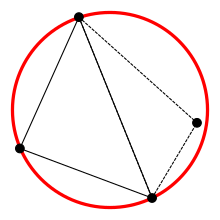
\includegraphics[width=\linewidth]{delaunay_mal}
  \caption{Vértice en el interior de una circunferencia circunscrita. No se cumple la condición de Delaunay}\label{fig:del_mal}
\endminipage\hfill
\minipage{0.32\textwidth}
  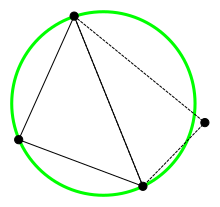
\includegraphics[width=\linewidth]{delaunay_bien}
  \caption{Vértice fuera de una circunferencia circunscrita. Se cumple la condición de Delaunay}\label{fig:del_bien}
\endminipage\hfill
\minipage{0.32\textwidth}%
  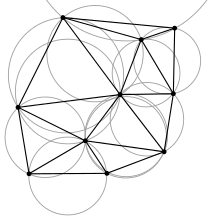
\includegraphics[width=\linewidth]{delaunay_bien_10pts}
  \caption{Triangulación de Delaunay aplicada a 10 puntos. Ninguna  de las circunferencias circunscritas contiene vértices en su interior}\label{fig:del_bien_10pts}
\endminipage
\end{figure}



El origen del nombre de la condición de Delauany se debe al matemático ruso Boris Nikolaevich Delone quien lo ideó en 1934 y tomó la forma francesa de su apellido, "Delaunay" como referencia a sus antecesores franceses.

%https://en.wikipedia.org/wiki/Point_cloud

Por otra parte, una peculiaridad o limitación respecto a las nubes de puntos tiene que ver con que la
información que representan es superficial, es decir, los puntos siempre pertenecen a la superficie del
objeto en cuestión ya que es el lugar donde la luz de los escáneres se llega, rebota y devuelve la
información correspondiente.

Otra desventaja inherente a las nubes de puntos es la interpretación de la información que contienen ya
que se ha explicado que está compuesta de un conjunto de objetos o puntos sin relación entre ellos. Es
aquí donde se requiere intervención del ser humano pues es su cerebro el que puede encontrar la similitud
entre una nube de puntos dada y el objeto o escenario que se supone que representa. Existe software capaz
de encontrar patrones y características para clasificar nubes de puntos pero nunca de forma
completamente fiable (ver aliasing)

El concepto de nube de puntos es eminentemente simple así como versátil y de gran utilidad. Esto se puede apreciar con gran multitud de aplicaciones del concepto de nube de puntos en el mundo real y es que este progreso tecnológico es un gran paso adelante para refinar procesos ya existentes, desde producción a nivel industrial hasta establecer las bases de la navegación de cualquier robot o vehículo.


Ejemplos
hacer nube de puntos simple con visor y poner captura
comparar con cosas como ... (tamaño, numero de puntos, color/no color...)


Se muestran a continuación varios ejemplos de nubes de puntos de diferentes características:

En primer lugar se tiene una sencilla nube de puntos que representa un conejo. Se ha tomado una captura desde uno de todos los posibles puntos de vista que ofrece una visión en 360º.
Un ejemplo algo más elaborado se recoge en la figura 1.5 en la que aparece una nube que representa un lobo. 
Otro ejemplo de mayor complejidad permite observar en la figura 1.6 un escaneo frontal de tres botes de plástico. En este caso, es obvio que las zonas vacías justo detrás de los botes son aquellos lugares donde los rayos de luz emitidos por el sensor no pueden llegar ya que los propios botes los bloquean lo cual sirve para que su superficie quede capturada. Además, se ha incluido un campo de color para cada punto.


\begin{figure}[!htb]
\minipage{0.32\textwidth}
  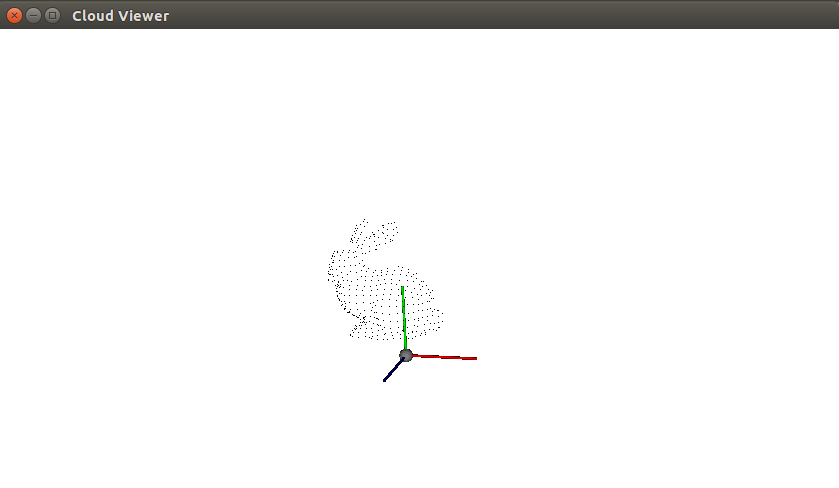
\includegraphics[width=\linewidth]{bunny_simple}
  \caption{Nube de puntos representando un conejo.
  Peso total de la nube: 10.6KB.
  Número total de puntos: 397.}\label{fig:bunny_simple}
\endminipage\hfill
\minipage{0.32\textwidth}
  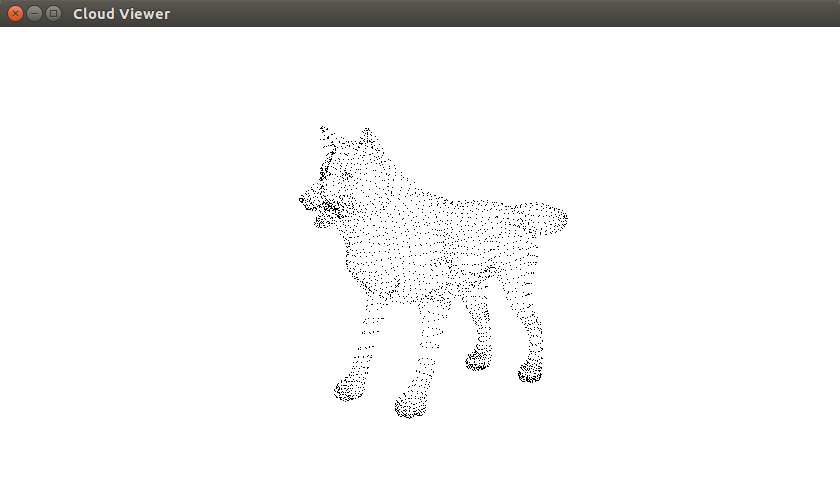
\includegraphics[width=\linewidth]{wolf}
  \caption{Nube de puntos representando un lobo.
  Peso total de la nube: 42.6KB.
  Número total de puntos: 3400.}\label{fig:wolf}
\endminipage\hfill
\minipage{0.32\textwidth}%
  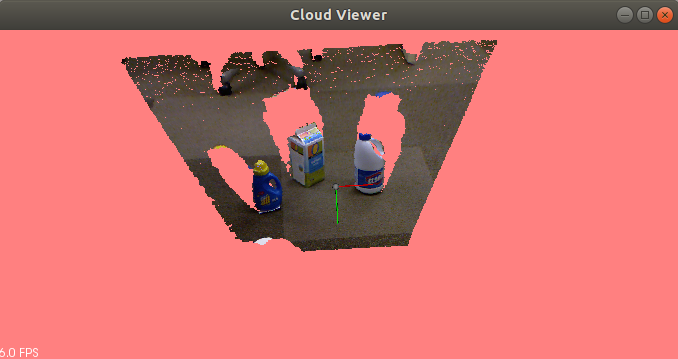
\includegraphics[width=\linewidth]{botes}
  \caption{Nube de puntos representando tres botes.
  Peso total de la nube: 2.43MB.
  Número total de puntos: 307200.}\label{fig:botes}
\endminipage
\end{figure}


%http://www.pointclouds.org/news/2013/01/07/point-cloud-data-sets/
%http://graphics.stanford.edu/data/3Dscanrep/
%http://kos.informatik.uni-osnabrueck.de/3Dscans/
%https://www.cc.gatech.edu/~turk/bunny/bunny.html

Una vez vistos ejemplos de nubes de puntos con la información suficiente para reconocer qué objeto representan sin más ayuda que la de los propios ojos, es momento de subir el nivel de complejidad para dar lugar a nubes de puntos como las que se muestran a continuación:

Se ha visto anteriormente una sencilla representación de un conejo con solamente 397 puntos. El nivel de detalle pude incrementarse a niveles del orden de decenas de miles de pintos tal y como es el caso de la figura 1.6 que representa una figura de arcilla de 7.5 pulgadas de alto con unos 69451 triángulos ya que se ha llevado a cabo la reconstrucción de la superficie. Además, en la figura 1.7 se aprecia el resultado si se añade información sobre color en cada punto.
Como consecuencia de añadir más información (más de 90 veces la cantidad de puntos y el color) se tiene en este caso un peso de 22MB con hasta 35947 puntos.
\begin{figure}[!htb]
\minipage{0.45\textwidth}
  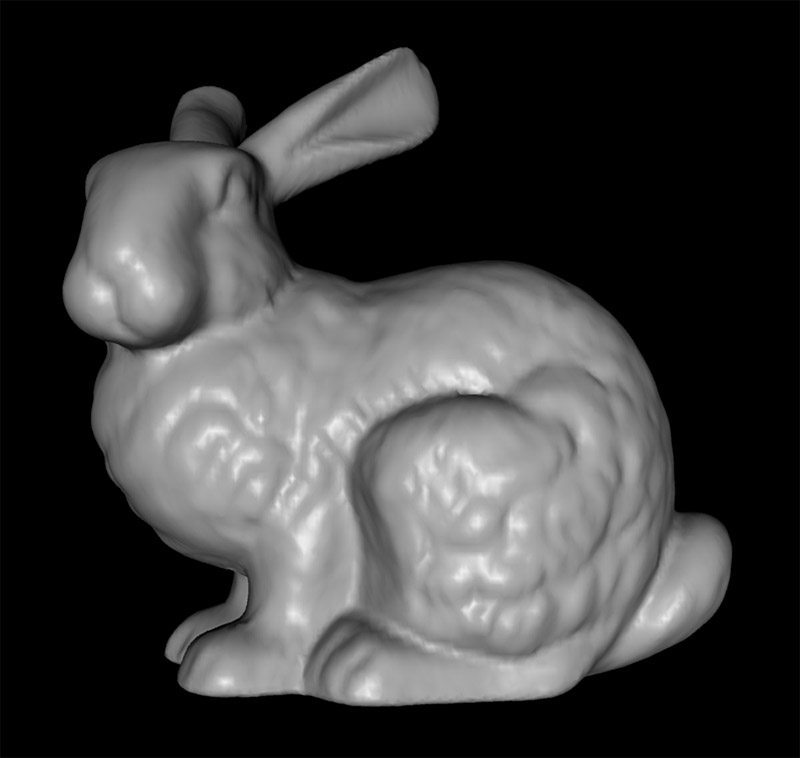
\includegraphics[width=\linewidth]{bunny}
  \caption{Nube de puntos con reconstrucción de superficie representando un conejo sin información de color.}\label{fig:bunny}
\endminipage\hfill
\minipage{0.45\textwidth}
  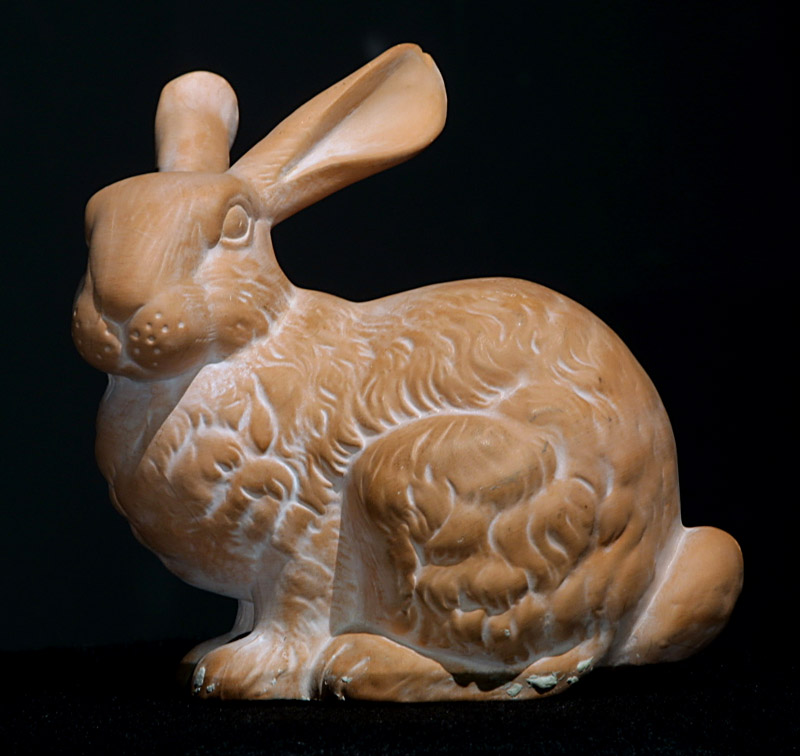
\includegraphics[width=\linewidth]{bunny_colored}
  \caption{Nube de puntos con reconstrucción de superficie representando un conejo con información de color.}\label{fig:bunny_colored}
\endminipage\hfill
\end{figure}
Esta nube de puntos proviene del departamento de computación gráfica de la universidad de Stanford e hicieron falta un total de 10 escaneos con el escaner Cyberware 3030 MS para llegar al resultado final. Para hacerse una idea del tipo de sensor utilizado, se tiene como dato relevante su precio de unos 10000 dólares (ebay) teniendo en cuenta además de que se trata de un sensor antiguo pues el escaneo se produjo en 1993.

Se pueden representar objetos más grandes y con mayor nivel de detalle tal y como se aprecia en la imagen x que representa un dragón construido con madera y resina y con un tamaño de aproximadamente 20cm x 8cm x 9cm.

\begin{figure}
\centering
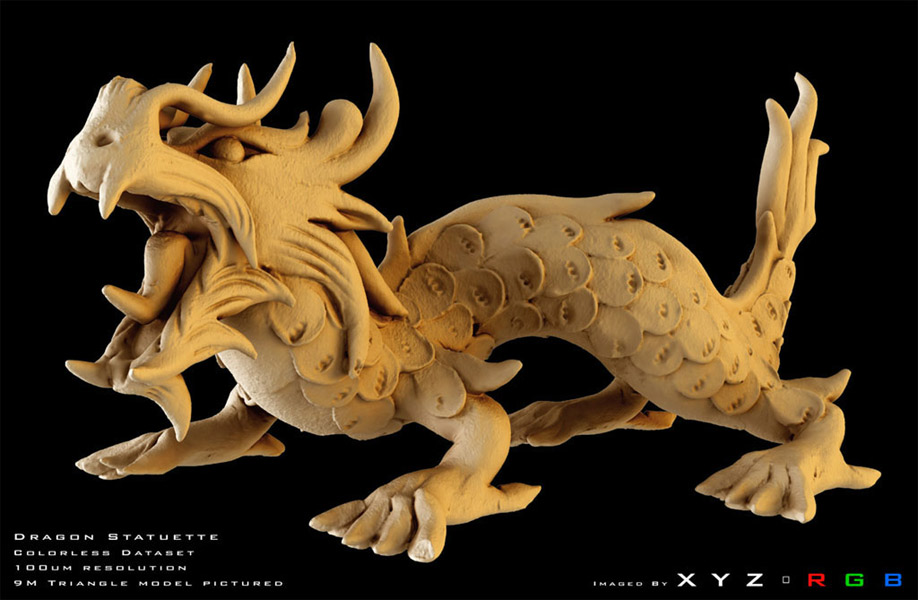
\includegraphics[scale=0.3]{dragon}
\caption{Nube de puntos con reconstrucción de superficie representando una figura de un dragón.}\label{fig:dragon}
\end{figure}

En este caso se han llevado a cabo 18 escaneos con una resolución de 100um o lo que es lo mismo, la separación entre puntos es del orden de 0,1mm. se dispone de un total de 3609455 puntos y 7218906 triángulos lo que implica un peso de 86MB para la nube reconstruida y descomprimida.
La nube de puntos se generó en el mismo laboratorio y con el mismo escaner que se ha mencionado en el caso anterior.

otro objeto de elevada complejidad que ha sido escaneado en las mismas condiciones que el dragón y el conejo es el ángel Lucy. Un total de 47 escaneos dan lugar a un resultado final de 14027932 puntos y 28055742 triángulos y para este caso un peso de 508MB tomando la nube de puntos reconstruida y descomprimida.

\begin{figure}
\centering
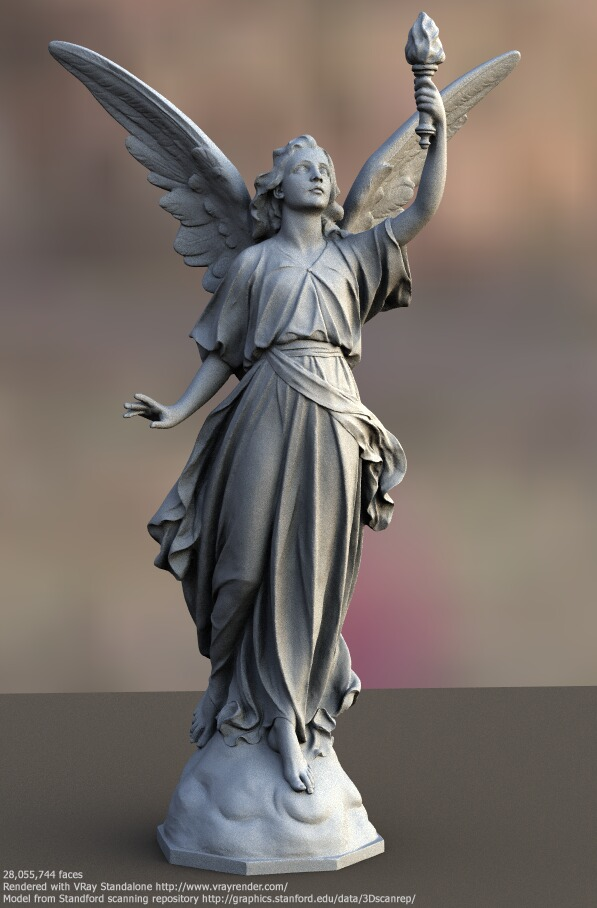
\includegraphics[scale=0.27]{angel_lucy}
\caption{Nube de puntos con reconstrucción de superficie representando una figura de un ángel.}\label{fig:angel_lucy}
\end{figure}

No solamente se pueden representar objetos mediante nubes de puntos sino entornos abiertos o interiores.

Johannes Schauer y Andreas Nüchter de la universidad de Würzburg, Alemania, tomaron la siguiente nube de puntos del mercado en la ciudad de Würzburg.
El escaner utilizado en el este caso es el Riegl VZ-400 y con un total de 6 escaneos se han conseguido 86585411 puntos conteniendo cada uno de ellos información sobre la reflectancia de la luz del sensor lo que se representa con puntos de diferente claridad ya que no hay información sobre color. Obviamente, un entorno exterior contiene mucha más información que un simple objeto por lo que esta nube de puntos tiene un peso de 5117MB descomprimida.

Cabe destacar que el sensor utilizado es bastante más potente que el anterior mencionado y tiene un precio de unos 80000 dólares.

\begin{figure}
\centering
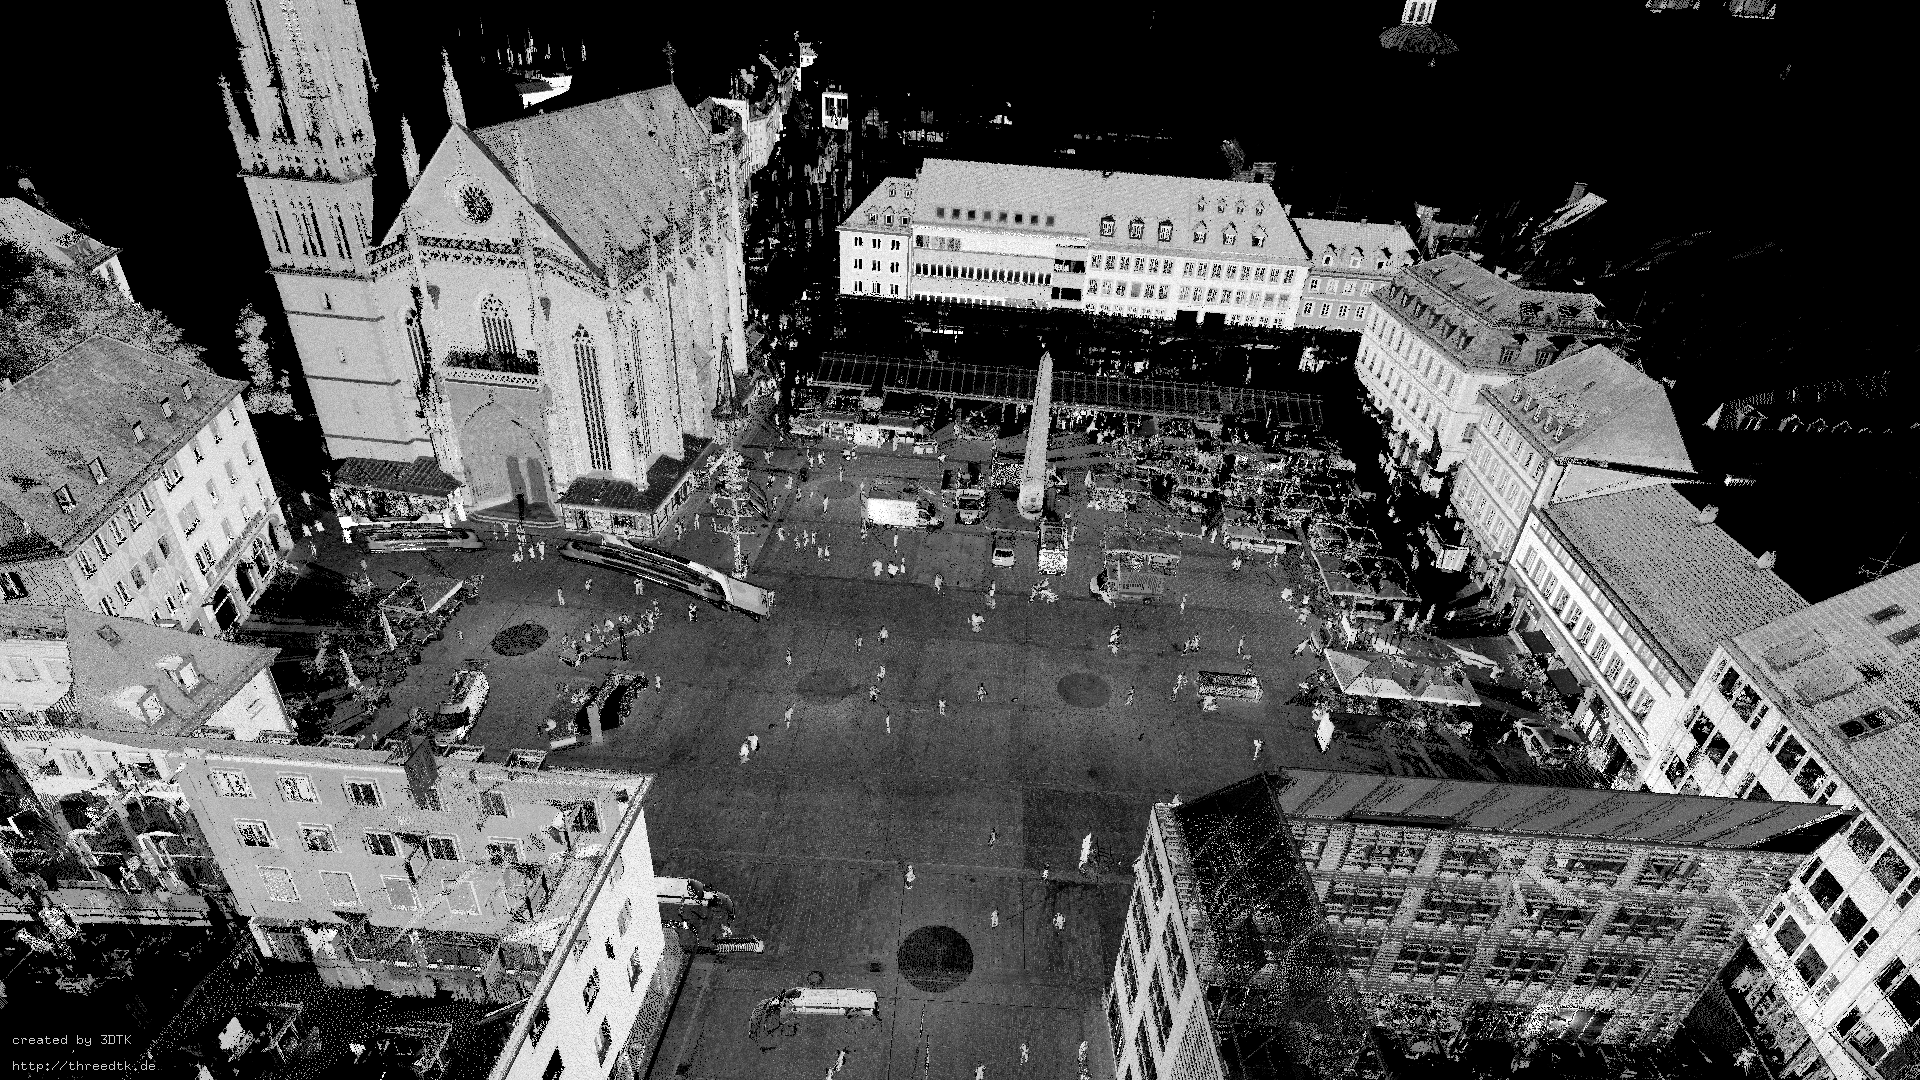
\includegraphics[scale=0.17]{wue_city2}
\caption{Nube de puntos con información de reflectancia de la luz que representa un mercado en Würzburg, Alemania.}\label{fig:wue_city}
\end{figure}

Por último, Dorit Borrmann obtuvo una nube de puntos que representa el interior del laboratorio de automática en la universidad de Jacobs, Bremen. Se pueden apreciar diferentes tipos de puntos para cada sección de la imagen ya que el sensor láser Riegl VZ-400 se encarga de representar información térmica y de profundidad mientras que las cámaras Optris PI IR y Logitech QuickCam 9000 Pro muestran información relacionada con el color.

\begin{figure}
\centering
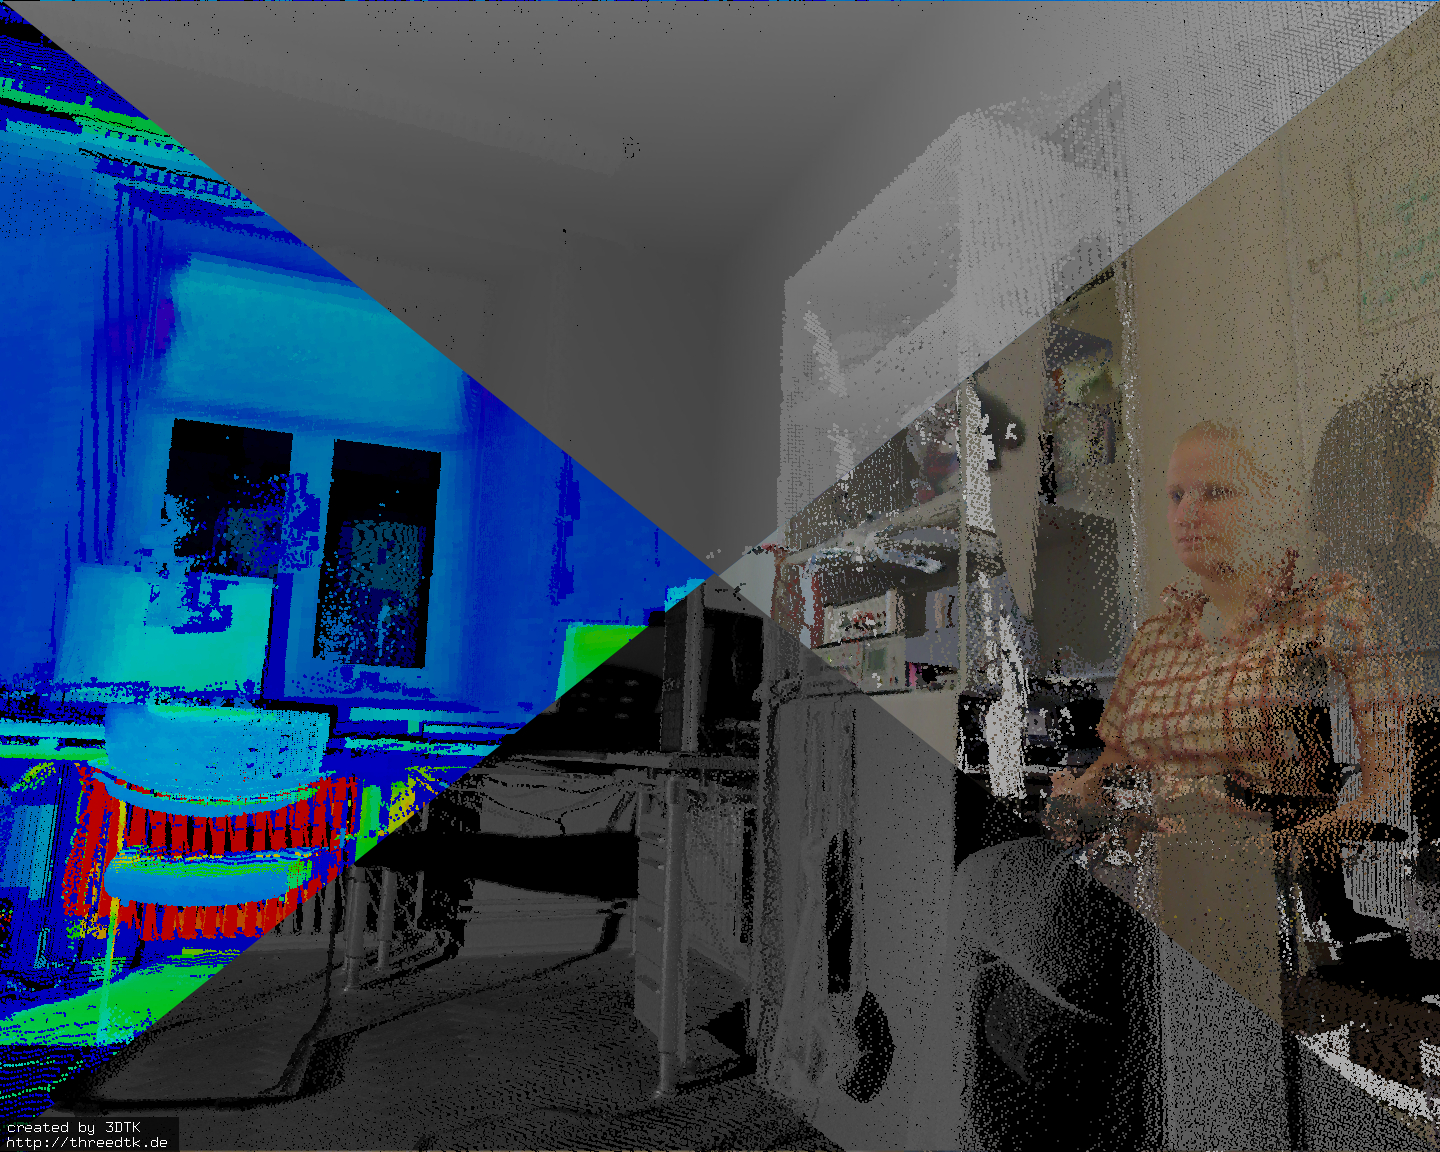
\includegraphics[scale=0.17]{joinedmodel}
\caption{Unión de cuatro nubes de puntos con información térmica, de color y reflectancia de la luz representando un entorno cerrado.}\label{fig:joined_model}
\end{figure}

Se hicieron un total de 9 escaneos en 40º cada uno lo que permite disponer de una imagen en 360º (la imagen mostrada es uno de los escaneos)




\section{Adquisición de información: Sensores y evolución}

La adquisición y almacenamiento de información es el primer paso para comenzar a trabajar con una nube de puntos. A pesar de tratarse de información relativamente sencilla como coordenadas respecto a un sistema de referencia, color y reflectividad, hay que tomar dicha información para miles o incluso millones de puntos tal y como se ha visto en ejemplos mostrados anteriormente como en el caso del ángel Lucy (figura ). Por lo tanto, el factor limitante del sensor en cuestión radica en cuánta y cuan variada información es capaz de percibir y almacenar.

En los últimos veinte años, se han hecho grandes progresos en lo que a sensores e refiere ya que actualmente se usan de sofisticadas cámaras y escaneres láser y se han dejado atrás los sensores basados en sonar o infrarrojos los cuales proporcionan a penas unos bytes de información sobre el entorno u objeto que tratan de representar.


Centrándose en los sensores láser, la adquisición de información cobra sentido cuando se tienen en cuenta la desviación de rayos de luz ya sea visible o infrarroja, por ejemplo.




 Para poder llevar a cabo el escaneo de objetos tridimensionales así como entornos, el escaneo laser o también conocido como lidar (light detection and ranging pero originalmente se conocía por la union de light and radar), 
es un procedimiento que se originó a principios de la década de los sesenta tras la invención del láser y permite medir distancias a un objetivo iluminándolo con pulsos láser y estudiando los tiempos de retorno y longitudes de onda de estos pulsos al rebotar y ser captados por un sensor conocido como rangefinder.

En la mayoría de los escaneres laser, la dirección de emisión del rayo de luz es constante por lo que para poder apuntar el haz hacia la dirección deseada se hace uso de espejos. Esto implica lanzar el láser contra un espejo y controlar éste con diferentes movimientos de rotación; en un eje para un movimiento unidimensional (un grado de libertad) o en dos ejes para un alcance espacial total quedando fija la posición del foco emisor(dos grados de libertad)

\begin{figure}[!htb]
\minipage{0.32\textwidth}
  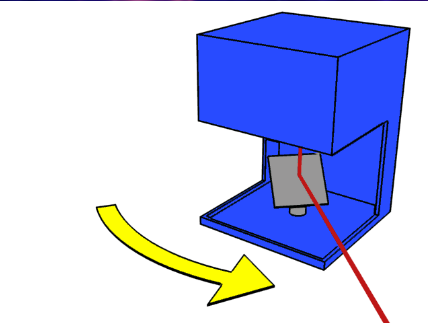
\includegraphics[width=\linewidth]{sensor_laser_espejo}
  \caption{Láser proyectado contra un espejo con un grado de libertad}\label{fig:sensor laser completo - espejo}
\endminipage\hfill
\minipage{0.32\textwidth}
  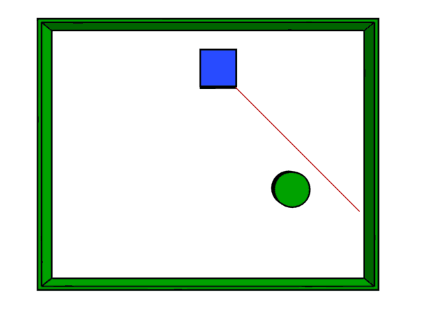
\includegraphics[width=\linewidth]{sensor_laser_vista_tope}
  \caption{Vista superior del sensor y las superficies que obstaculizan el haz de luz: objeto y recinto en el que se encuentra}\label{fig:sensor laser completo - vista tope}
\endminipage\hfill
\minipage{0.32\textwidth}
  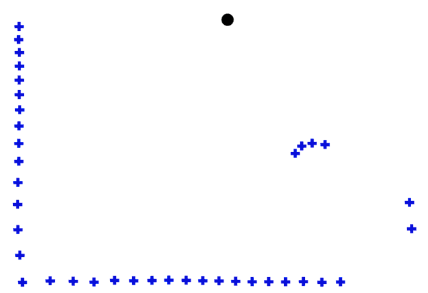
\includegraphics[width=\linewidth]{sensor_laser_resultado}
  \caption{Conjunto de puntos obtenidos tras el esacaneo pertenecientes al objeto en el interior del recinto y las limitaciones espaciales del mismo.}\label{fig:sensor laser completo - resultado}
\endminipage
\end{figure}

Una alternativa para controlar el rayo láser en dos dimensiones incumbe el uso de dos espejos montados en ejes ortogonales y entonces hacer movimientos de rotación entorno a un eje para cada uno de los espejos.

\begin{figure}
\minipage{0.45\textwidth}
  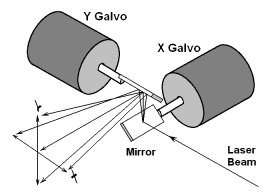
\includegraphics[width=\linewidth]{sensor_dos_espejos}
  \caption{Uso de dos espejos con un grado de libertad en cada uno y accionados con galvanómetros}\label{fig:sensor dos espejos}
\endminipage\hfill
\minipage{0.45\textwidth}
  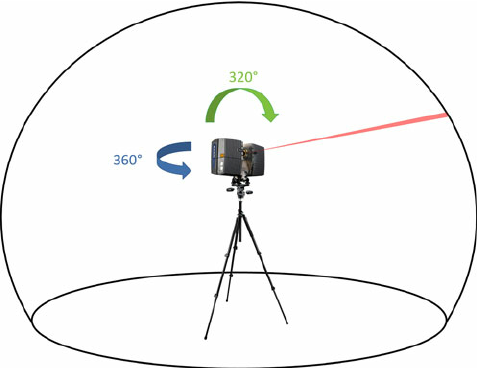
\includegraphics[width=\linewidth]{movimiento_lidar_2D}
  \caption{Sensor lidar con dos grados de libertad.}\label{fig:movimiento lidar 2D}
\endminipage\hfill

\end{figure}


para sistemas más sofisticados todavía, se requiere el posicionamiento espacial del foco emisor de rayos lo cual se consigue con un sistema de lentes servo controladas conocido como focus shifter o z-shifter

la forma más común de mover los espejos es mediante el uso de un motor eléctrico o un galvanómetro para el más sencillo de los casos. Se pueden utilizar también actuadores piezoeléctricos o magnetorresistivos para una mayor velocidad angular pero a costa de menores ángulos máximos de desplazamiento


De este modo, al ser capaz de medir la distancia que hay desde el punto de emisión de los rayos de luz hasta la superficie en la que rebotan, el sensor puede detectar rápidamente formas definidas de objetos, edificios o paisajes considerando en conjunto de puntos detectados tal y como se ha mostrado en ejemplos del apartado anterior concepto de nube de puntos (hipervínculo)

Por lo general, hay dos tipos de lidar:
método coherente e incoherente o también conocido como detección de energía directa.
El método incoherente mide cambios en la amplitud de la onda emitida pues al rebotar e interactuar con el ambiente su nivel de energía varía.

imagen cambio amplitud

El método coherente es más apropiado para medir diferencias en la frecuencia de la onda y utiliza (Optical heterodyne detection) lo que le permite operar a potencias mucho más bajas a costa de utilizar un equipamiento mucho más complejo (more complex transceiver requirements)

imagen cambio fase


En ambos modelos se pueden usar dos tipos diferentes de pulsos: micropulsos y sistemas de alta energía.
los micropulsos surgen de la elevada capacidad computacional de las computadoras actuales. Esto deriva en un láser de baja potencia (del orden del microjulio) que es clasificado como seguro al ojo permitiéndose su uso bajo escasas medidas de precaución 

Por otra parte, los sistemas de alta energía, requieren medidas de seguridad más estrictas y se usan principalmente para fines de investigación atmosférica pues permite tomar medidas como la altura, número de capas y densidad de las nubes, propiedades de las partículas en las nubes, temperatura, presión, concentración de gases, o humedad.



Para cada pulso de luz emitido se detecta un punto en concreto lo que hace pensar que para poder crear nubes con millones de puntos la velocidad de generación de los pulsos ha de ser elevada. En el caso de lidar se pueden emitir hasta 150000 pulsos en un segundo.

En cuanto a los componentes necesarios para cualquier sistema lidar 
...

Pero ¿Cómo se pueden medir distancias utilizando luz? el concepto entorno al que el escaner laser gira es el tiempo de vuelo. Esto quiere decir que se utiliza un dispositivo (range finder) capaz de medir con precisión el tiempo que transcurre desde que se emite un pulso de luz hasta que vuelve otra vez al mismo tras rebotar sobre el objeto que desea detectarse. Considerando entonces que la velocidad de la luz es una constante conocida, c, la distancia del escaner a un punto en concreto donde rebota un determinado pulso de luz puede determinarse como:

ecuacion d= c*t/2

Nótese que c*t es la distancia que hay entre el escaner y el objeto duplicada ya que t es el tiempo total desde la emisión del pulso de luz hasta la recepción. Por tanto, tomando la mitad del tiempo total de vuelo se obtiene la medida deseada que es la distancia del escaner al objeto.

Retomando la idea de que la velocidad de la luz es una constante, la única variable en el cálculo de la distancia es el tiempo de vuelo. Téngase por ejemplo una distancia de 30cm desde el sensor hasta el objeto que desea capturarse.Esto implica que la resolución del reloj integrado en el sensor ha de ser cuanto menos elevada:

%0,3m/3*10^8=1ns=0,000000001s, en ese tiempo...

Se ha desvelado de esta forma una desventaja del concepto de tiempo de vuelo, se necesita equipamiento muy preciso y fiable lo que se traduce en complejidad y elevadas inversiones económicas.

Pero dando la vuelta a esta desventaja, es decir, cuando se trata de escanear objetos en la lejanía como puede ser un edificio o paisaje,la resolución requerida por parte del reloj se reduce dando así medidas más fiables. Además, considerando de nuevo la velocidad de la luz como una constante, no importa la distancia a la que se encuentre el objeto salvo por cuestiones de difracción y absorción del pulso de luz en el ambiente, por ejemplo , por la presencia de humedad.

Una aplicación muy extendida del lidar es el reconocimiento de terreno. Para ello se integra el sensor en una aeronave y se capturan los puntos correspondientes al terreno sobrevolado. Esta aplicación es útil para generar modelos digitales de elevación.
Como contrapartida, hay que tener en cuenta que el sensor tiene una posición variable respecto al terreno ya que va embarcado en una aeronave. Para considerar esto en el resultado final de la nube de puntos generada, se ha de disponer de un sistema de navegación, para el posicionamiento del sensor con GPS por ejemplo, así como de una unidad de medidas inerciales, para obtener información sobre la posición angular del sensor según los tres ejes espaciales, es decir, medir los movimientos yaw, pitch y roll.

 
\begin{figure}
\minipage{0.45\textwidth}
  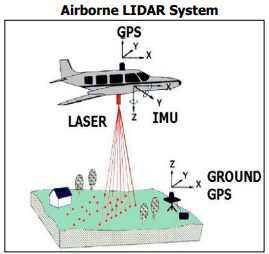
\includegraphics[width=\linewidth]{airborne_lidar}
  \caption{Esquema de utilización del método lidar en una aeroanve}\label{fig:airborne_lidar}
\endminipage\hfill
\minipage{0.45\textwidth}
  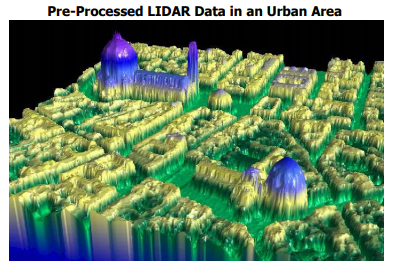
\includegraphics[width=\linewidth]{airborne_city}
  \caption{Entorno urbano recreado con el método lidar}\label{fig:airborne_city}
\endminipage\hfill

\end{figure}

Este método combina precisión y versatilidad ya que puede valerse de luz visible, infrarroja o ultravioleta para lanzarla contra objetivos de diversos tipos de materiales como metal, cerámica, aerosoles, terreno (rocas y tierra) e incluso se puede llegar al nivel molecular. 
 



Sin embargo no se realiza un único escaneo ya que el propio concepto implica que el objeto bloquea los rayos de luz por lo que la cara frontal, de la que sí se obtiene información, impide a la luz llegar a la cara posterior. El factor clave es entonces el hecho de que estos rayos de luz puedan llegar a toda la superficie del objeto que se quiere analizar, es decir, accesibilidad física del sensor.
De este modo, independientemente del sensor o método que se utilice, es imposible recolectar
información sobre superficies no visibles o lo que es lo mismo, con un solo escaneo.


imagen botes por ejemplo


Como consecuencia, es necesario llevar a cabo varios escaneos desde diferentes puntos de vista y
ponerlos en conjunto conociendo con precisión la posición del sensor en cada escaneo para poder llevar a cabo lo que se conoce como alineamiento de nubes de puntos, concepto que se explicará con más detalle posteriormente.






%https://upload.wikimedia.org/wikipedia/commons/c/c0/LIDAR-scanned-SICK-LMS-animation.gif
%https://www.engineering.com/AdvancedManufacturing/ArticleID/12390/Quality-Basics-How-Does-3D-Laser-Scanning-Work.aspx
%https://en.wikipedia.org/wiki/Laser_scanning
%http://www.2grobotics.com/wp-content/uploads/2017/03/sonarvslaser.pdf
%http://www.lidar-uk.com/how-lidar-works/
%http://elm-chan.org/works/vlp/report_e.html
%http://www.ionix.fi/en/technologies/laser-processing/laser-marking/

Disponer de complejas, fiables y robustas representaciones del mundo real tiene no es tan sencillo como pueda parecer puesto que estos sensores suelen tener un precio prohibitivo para la mayoría de los interesados ya sean particulares o incluso empresas con un poder adquisitivo considerable. Sin embargo, las tornas han cambiado desde que han aparecido en el mercado ciertos sensores 3D como por ejemplo el sensor Kinect de la consola Xbox360 de Microsoft. Este sensor está basado en la tecnología PrimeSense y aunque puede trabajar con nubes de puntos en tiempo real e imágenes en 2D su precio no supera los 150\$. De este modo se ha producido un gran paso adelante en cuanto a los impedimentos relacionados con la adquisición, mantenimiento y delicadeza del hardware que traduce el mundo real a nubes de puntos.

\section{Procesamiento software de información }
\section{objetivos}
Una vez estudiado el hardware necesario se precisa ahora de un mecanismo para trabajar con la inmensa cantidad de información que aportan los sensores. 

El software existente para dicha tarea es diverso y no siempre gratuito. Como ejemplos se tienen:
\begin{list}{-}
\item 3DF Zephyr
\item RealityCapture
\item Agisoft Photoscan
\item Point cloud tool

\textit{describir brevemente y mencionar impedimentos de precio, limitaciones etc
}
\end{list}




Es aquí donde entra en juego una librería de código abierto llamada PCL (insertar imagen-web) siglas que en inglés representan Point Cloud Library, traducible como librería de nubes de puntos.

\textit{Definir qué es pcl, historia, extensión
http://pointclouds.org/
paper: 3D is here}


\section{Descripción de herramientas}
\subsection{Herramientas hardware}
\subsection{Herramientas software}


Generar un programa capaz de obtener keypoints a partir de una nube de puntos
Croscompilar usando las herramientas de xilinx 
Enviar ejecutable a la placa y ejecutar el programa
(optimización)


\chapter{Herramientas empleadas para la realización del proyecto}

\section{Introducción}
Habiendo tratado en el capítulo anterior el fundamento teórico que concierne a las nubes de puntos y el procesamiento software de las mismas se procede en este capítulo a explicar con mayor profundidad las herramientas necesarias para cumplir los objetivos propuestos para el presente trabajo.



\section{Descripción de herramientas para desarrollar el trabajo}
Para realizar el presente trabajo se requieren herramientas que pueden clasificarse en dos tipos: software y hardware.

\subsection{Herramientas software}
\subsubsection{Máquina virtual}
Se hace uso de una máquina virtual con Ubuntu\cite{ubuntu} 18.04.1 64 bits ya que es un sistema operativo que facilita la instalación y uso de PCL y otras librerías, no como Windows.
Por lo tanto, a partir de este punto, salvo que se mencione lo contrario, el sistema de archivos e instrucciones ejecutadas por línea de comandos así como demás características propias de diferentes sistemas operativos se refieren a un sistema operativo basado en Linux.
\\
\\
La máquina virtual se crea haciendo uso del software VirtualBox\cite{virtualbox} el cual facilita la creación y personalización de máquinas virtuales no solamente basadas en Linux sino con cualquier otro sistema operativo.

%https://www.virtualbox.org/
\subsubsection{Instalación de PCL sobre un sistema basado en Linux}
Una vez se dispone de la máquina virtual, es necesario instalar las librerías de PCL\cite{pcl_installation}. Para ello se visita la web oficial de PCL pues ésta ofrece las instrucciones adecuadas. Para poder instalar PCL en linux se deben ejecutar los siguientes comandos:

%http://pointclouds.org/downloads/

\begin{verbatim}
sudo add-apt-repository ppa:v-launchpad-jochen-sprickerhof-de/pcl
sudo apt-get update
sudo apt-get install libpcl-all
\end{verbatim}

La primera instrucción añade al sistema el repositorio en el que se encuentra la librería, el segundo busca actualizaciones disponibles y por último se procede a la instalación de todos los archivos actualizados.
\\
\\
Estas mismas instrucciones sirven para instalar PCL en el sistema embebido ya que dispone del un sistema operativo Debian basado en Linux.
\\
\\
Cuando la instalación está completa, se generan una serie de carpetas en el directorio /usr/include:

\begin{itemize}
\item[•]pcl-1.8: Es la versión 1.8 de la librería de PCL. Contiene en su interior la carpeta pcl que con todos los módulos de PCL estructurados correctamente.
\item[•]eigen3: Librería eigen que se encuentra bajo la carpeta Eigen dentro de este directorio.
\item[•]FLANN: Librería FLANN que se encuentra bajo la carpeta flann dentro de este directorio.
\item[•]vtk-x: versión x de la librería vtk 
\end{itemize}

\subsubsection{Vivado Design Suite HLx Editions}
Ya está instalado PCL en el sistema, ahora falta adquirir una herramienta para síntesis de alto nivel.
\\
\\
La síntesis de alto nivel, del inglés High Level Synthesis (HLS) es un proceso de diseño automático que interpreta una descripción algorítmica en software de un comportamiento deseado y crea hardware digital que lo implementa.
\\
\\
La síntesis comienza con una descripción en alto nivel del problema o comportamiento que desea reproducirse. Para ello se puede utilizar uno de los varios lenguajes de programación en alto nivel como C o C++. Este código es entonces analizado y programado para ser compilado en lo que se conoce como un Register Transfer Level (RTL), es decir, la abstracción del diseño que modela un circuito digital síncrono en sus señales entre registros y las operaciones realizadas sobre ellas.  El diseño de hardware puede ser generado a diferentes niveles de abstracción: puertas lógicas, registros y algoritmos. Se aprecia en la figura \ref{fig:circuito} un diseño hardware a nivel de registro de un circuito inversor.
\begin{figure}[!htb]
\centering
\includegraphics[scale=0.25]{circuito}
  \caption{Circuito digital síncrono que actúa como un inversor de la señal de entrada.}\label{fig:circuito}
\end{figure}

El RTL queda definido mediante un Hardware Description Language (HDL) del inglés, lenguaje de descripción de hardware como VHDL o Verilog. Para el caso del ejemplo anterior y tomando VHDL como el lenguaje de descripción, la definición del circuito de la figura \ref{fig:circuito} queda como:

\begin{lstlisting}[language=VHDL,breaklines]
D <= not Q;
 
process(clk)
begin
    if rising_edge(clk) then
        Q <= D;
    end if;
end process;
\end{lstlisting}


El objetivo de la síntesis en alto nivel es permitir a los diseñadores construir y verificar hardware de forma eficiente así como el de dotarles de mayor control y optimización sobre sus diseños con la facilidad añadida de poder definirlos mediante lenguajes de alto nivel de abstracción mientras la herramienta realiza la implementación del RTL de forma automática.
\\
\\
Para realizar la síntesis de alto nivel se elige la herramienta vivado HLS de Xilinx. Accediendo a la web oficial de descargas\cite{vivado_descarga} se puede descargar la versión deseada de este software ya sea como un archivo comprimido un instalador web para mayor comodidad. En este caso se elige la versión 2017.1
\\
\\
Haciendo uso del mencionado software de Xilinx, se define en un lenguaje de programación de alto nivel, por ejemplo C++, un comportamiento que se implementa como una función con sus argumentos, operaciones internas y un valor de retorno. Además, deben definirse unos ``pragmas'', es decir, una región de código considerada como un protocolo y en el que Vivado HLS no introduce ninguna señal de reloj excepto si se indica explícitamente. Una región definida como un protocolo puede ser utilizada para especificar de forma manual una interfaz de conexión a otros bloques hardware con el mismo protocolo de entrada/salida de señales. Esto implica que, por ejemplo, dado un bloque hardware, se pueden definir dos buses: un bus IN que contiene todas las señales de entrada al bloque y un bus OUT que contiene todas las señales salientes.


%https://www.xilinx.com/support/download.html
%https://www.xilinx.com/products/design-tools/vivado/integration/esl-design.html

\subsection{Herramientas hardware} \label{herraminetas_hardware}
La principal herramienta hardware de la que se dispone y sobre la cual se comprobarán los resultados de la aplicación de los objetivos del presente trabajo es la placa de desarrollo Pynq-Z1\cite{pynq} que se puede ver en la figura \ref{fig:pynq}. Se trata de una placa de bajo coste y ampliamente utilizada en universidades y centros de investigación.

\begin{figure}[H]
\centering
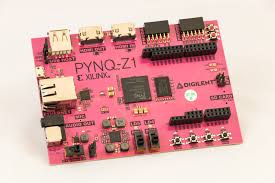
\includegraphics[scale=1.0]{pynq}
  \caption{Placa de desarrollo Pynq-Z1 de Xilinx.}\label{fig:pynq}
\end{figure}

Esta placa dispone de un System on Programmable Chip (SoPC) del inglés sistema en chip programable, del modelo Zynq xc7z020clg400-1. Un sistema en chip programable es la combinación de núcleos de procesamiento de una CPU (Central Processing Unit o unidad central de procesamiento) con hardware personalizado que se implementa normalmente con una FPGA y bloques de memoria.
\\
\\
Una FPGA, siglas del inglés ``Field Programmable Gate Array'' o matriz de puertas programables es un dispositivo programable que contiene bloques de lógica cuya interconexión y funcionalidad pueden ser reconfiguradas en tiempo de ejecución.
\\
Además, una FPGA dispone de dos capas: aplicación y configuración. La primera se compone de todos sus recursos hardware que han de ser configurados e interconectados haciendo uso de la segunda, la capa de configuración en la que se carga un ``bitstream'' es decir un archivo de configuración que se puede generar, entre otras formas, haciendo uso del programa Vivado de Xilinx y que permite para cada ``bitstream'' que se cargue, dotar a la FPGA de diferentes funcionalidades.
\\
\\
Volviendo al ámbito de un SoPC, los núcleos del procesador pueden ser ``hard'' (duros) o ``soft'' (blandos): los primeros son permanentemente embebidos en silicio mientras que los segundos se implementan usando recursos de una FPGA. 
\\
Los núcleos duros ofrecen mucho rendimiento y bajo consumo pero son poco flexibles en cuanto a las operaciones que pueden realizar. Éstos forman el Processing System (PS) dentro del SoPC para rutinas software y operaciones relacionadas con sistemas operativos a diferencia de la FPGA que conforma la Programmable Logic (PL) que sirve para implementar lógica de alta velocidad y aritmética.
\\
La PS dispone en este caso de un sistema operativo Debian basado en el kernel Linux.
\\
\\
%http://ati.ttu.ee/~alsu/05_SoPC.pdf
Algunas de las características principales del PS del SoPC mencionado son:

\begin{itemize}
\item[•] Un procesador Cortex-A9 de dos núcleos a 650MHz y arquitectura ARM, memoria caché de nivel 1 con 32KB pra instrucciones y 32KB para datos, memoria caché de nivel 2 y 512KB y memoria en chip de 256KB.
\item[•] Controlador de memoria DDR3 con 8 canales DMA y 4 puertos esclavos AXI3 de alto rendimiento
\item[•] Controladores de periféricos con elevado ancho de banda: Ethernet 1G, USB 2.0 y SDIO 
\item[•] Controlador de periféricos de gran ancho de banda: SPI, UART, CAN, I2C
\item[•] 630KB de memoria RAM
\item[•] Programable con JTAG, flash Quad-SPI y tarjeta micro SD
\end{itemize}


En cuanto al PL del SoPC:
\begin{itemize}
\item[•] 13300 secciones de lógica cada una de ellas con 4 Look-up Tables de 6 entradas y 8 Flip-Flops
\item[•]630KB de block RAM
\item[•] 4 unidades de administración de la señal de reloj
\item[•] 220 secciones de lógica para procesamiento de señales digitales (DSP)
\item[•] Conversor analógico-digital integrado en chip (XADC)

\end{itemize}

\section{Conclusiones}
Con el cierre del presente capítulo terminan las explicaciones fundamentales tanto de teoría como de herramientas que permiten estructurar el TFG.
\\
En el siguiente capítulo se mostrarán las primeras tareas que giran entorno a la librería PCL para así poder visualizar nubes de puntos y extraer keypoints de las mismas.


\chapter{Desarrollo de un pipeline de visualización y procesamiento de nubes}

\section{Introducción}
Dejando asentado el fundamento teórico ofrecido por capítulos anteriores, se plantea a continuación la posibilidad de no solamente disponer de un sistema de visión funcionando sobre un dispositivo embebido sino además poder realizar mediciones sobre el rendimiento de los algoritmos de PCL involucrados. Para ello, se crean dos programas de modo que, dada una nube de puntos, uno de ellos pueda visualizarla y otro extraiga keypoints.
\\
Como ya se ha mencionado en el primer capítulo de la memoria, el objetivo principal del trabajo es la reproducción de un algoritmo de extracción de keypoints sobre un sistema embebido. Como objetivo adicional, se reproduce también la visualización de nubes de puntos usando PCL. Es por esto por lo que se crean los dos programas mencionados y que se explican en el presente capítulo. Se recuerda que la relación entre ambos es la de poder visualizar los resultados del programa de extracción de keypoints en un ordenador de propósito general.
\\
Se describe a partir de este punto el trabajo técnico realizado por el propio autor como desarrollo del proyecto.

\section{Compilación de bibliotecas PCL mediante CMake}
En este apartado se pretende motivar el uso de CMake para compilar bibliotecas de PCL y ver cómo se lleva a cabo. 
\\
CMake se trata de un conjunto de herramientas diseñado para construir, probar y empaquetar software de forma automática. El control del proceso de compilación es posible gracias a unos ficheros de configuración sencillos e independientes de la plataforma de trabajo en la que se usan y que son llamados CMakeLists.txt. A partir de éstos, CMake genera makefiles nativos así como espacios de trabajo que pueden usarse en el entorno de trabajo deseado. Se aprecia entonces gran flexibilidad en esta forma de compilar librerías que son para el caso las de PCL.
\\
\\
Para la compilación de las librerías PCL se parte de un directorio de trabajo llamado, por ejemplo, ``prueba'' en el que se encuentran:

\begin{itemize}
\item[•]prueba.cpp: Es el código escrito en C++ y que no tiene ninguna funcionalidad de por sí. 

\item[•]CMakeLists.txt: Es el fichero de configuración que carga los módulos necesarios de la librería PCL y que mediante el cual, CMake, genera el makefile apropiado. Un ejemplo de CMakeLists.txt es el siguiente\cite{ejecutable}:

\begin{lstlisting}
cmake_minimum_required(VERSION 2.6 FATAL_ERROR)	
project(PRUEBA)	
find_package(PCL 1.3 REQUIRED)	
include_directories(${PCL_INCLUDE_DIRS})	
link_directories(${PCL_LIBRARY_DIRS})	
add_definitions(${PCL_DEFINITIONS})	
add_executable(pcd_write_test pcd_write.cpp)	
target_link_libraries(pcd_write_test ${PCL_LIBRARIES})	
\end{lstlisting}

Donde se indica por orden: 

\begin{itemize}
\item[1)]Mínima versión de CMake requerida
\item[2)]Nombre del proyecto, para el caso, ``PRUEBA''.
\item[3)]Búsqueda de librería PCL con versión mínima 1.3
\item[4)]Inclusión de directorios de los encabezamientos de la librería PCL
\item[5)]Inclusión de directorios de instalación de PCL y las librerías auxiliares
\item[6)]Definiciones del preprocesador y banderas de compilación
\item[7)]Nombre del ejecutable 
\item[8)]Se indica al linker la librería de PCL
\end{itemize}

\item[•]build: Es una carpeta donde almacenar el ejecutable generado a partir del código fuente, el makefile y demás archivos necesarios para la compilación.
\end{itemize}

Una vez creados el código fuente, CMakeLists.txt y build, se ejecutan los siguientes comandos para generar el ejecutable:

$$cd \;\; build$$
$$sudo \;\; cmake \;\; ..$$
$$sudo \;\; make$$
\\
Si todo sale bien, aparecerá un ejecutable en la carpeta build con el nombre indicado en CMakeLists.txt
\\
\\
Puesto que el código escrito en cualquier lenguaje de programación puede resultar complicado de transmitir, la forma de proceder para conseguir dicho objetivo será la siguiente: en primer lugar se explicará en alto nivel el programa en cuestión sin necesidad de leer código y haciendo uso de flujogramas u otros métodos que se consideren adecuados. Después, habiendo entendido la funcionalidad del programa, se explicarán las partes más relevantes del código que lo compone con el nivel de detalle adecuado en cada momento. Para esto, también aparecerán flujogramas así como la explicación de las partes más importantes.

 
\section{Programa de visualización de nubes de puntos}\label{visualizacion}
Tal y como se ha mencionado en el apartado de objetivos del presente trabajo, la visualización de nubes se considera un hito transversal pero que a la vez involucra todo el proyecto ya que es la parte más amigable al ojo humano para estudiar resultados. De este modo se aprovecha el libre uso de la documentación y los tutoriales ofrecidos por PCL\cite{modulo_io} para modificar el código a favor de los objetivos planteados en el TFG.
%http://pointclouds.org/documentation/tutorials/
\\
\\
Para la visualización de nubes se parte de un ejemplo disponible en la documentación de PCL\cite{ejemplo_visualizacion} que permite ver la representación espacial de la nube de puntos así como añadir esferas en cualquiera de ellos y así distinguirlos de los demás.
\\
De este modo, el autor del presente trabajo ha introducido las modificaciones necesarias para no solamente visualizar una nube de puntos como tal, sino resaltar en ella sus puntos SIFT.
\\
\\
Se recuerda que la visualización de nubes no puede llevarse a cabo en el sistema embebido ya que no dispone de interfaz gráfica.

\subsubsection{Explicación en alto nivel}
Para la visualización de una nube de puntos con o sin sus puntos SIFT se necesita en primer lugar hacer uso del módulo IO que permite leer nubes en formato PCD. De esta forma se puede:

\begin{itemize}
\item[•]Leer una única nube de puntos para mostrarla por pantalla como tal.
\item[•]Leer dos nubes de puntos, en primer lugar una nube de puntos A y posteriormente una nube de puntos B que contiene los puntos SIFT de la nube A. De esta forma, se resaltan visualmente los puntos contenidos en la nube B y se visualiza junto a la nube A de modo que se pueden ver en conjunto todos los puntos de la nube original, tanto los que son keypoints como normales. 
\end{itemize}

Cuando la nube está cargada, utilizando el módulo visualization, se crea una nueva ventana que hace de visualizador y en la que aparecen los tres ejes coordenados XYZ y el conjunto de puntos que conforman la nube situados en el espacio respecto al origen de los mencionados ejes. Cuando el usuario lo desee, puede cerrar la ventana que el programa ha creado para terminarlo.
\\
Este conjunto de operaciones se muestran en su explicación en alto nivel en forma de flujograma en la figura \ref{fig:visualization_all_diagram}

\begin{figure}
\centering
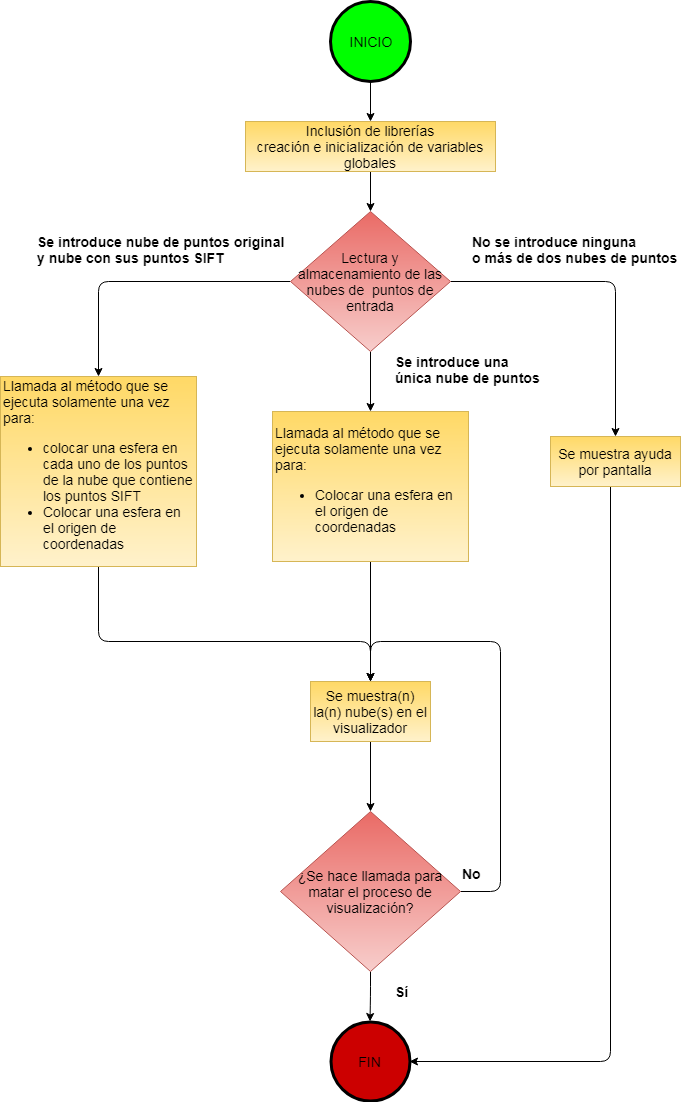
\includegraphics[scale=0.5]{visualization_all_diagram}
\caption{Flujograma del proceso de visualización de nubes de puntos.}\label{fig:visualization_all_diagram}
\end{figure}


\subsubsection{Explicación en bajo nivel}
Puesto que el código del programa de visualización no es objeto de estudio ni aceleración se prescinde de su explicación detallada.

\iffalse
El ejecutable generado dentro de la carpeta build se llama $visualization$ y para hacer funcionar el programa se han de ejecutar estos comandos, que en caso de querer visualizar una nube sin sus puntos SIFT:

$$./visualization \;\; nube1.pcd$$

y para visualizar una nube y sus keypoints:
$$./visualization \;\; nube1.pcd \;\; nube1\_keypoints.pcd$$

En relación al código que implementa esta funcionalidad, en primer lugar se cargan las librerías de $iostream$ para las funcionalidades básicas de C++ y determinados módulos de la librería PCL: $IO$ para la lectura de nubes, $cloud\_viewer$ del módulo $visualization$ para la visualización de nubes y $parse$ del módulo $console$ para poder evaluar los argumentos introducidos por la consola de comandos.
Además, se crea la instancia $sift\_cloud$ de la clase $PointCloud$, es decir, una nube de puntos donde almacenar y modificar (resaltar puntos) la nube que contiene keypoints.

\begin{lstlisting}[language=C++,breaklines]
#include <iostream>
#include <pcl/visualization/cloud_viewer.h>
#include <pcl/io/io.h>
#include <pcl/io/pcd_io.h>
#include <pcl/console/parse.h>
pcl::PointCloud<pcl::PointXYZRGBA>::Ptr sift_cloud (new pcl::PointCloud<pcl::PointXYZRGBA>);
\end{lstlisting}

A continuación se implementa el método que muestra ayuda por pantalla.

\begin{lstlisting}[language=C++,breaklines]
void 
printUsage (const char* progName)
{
  std::cout << "\n\nUsage: "<<progName<<" <cloud.pcd> (optional <SIFTpoints.pcd>)\n\n";
}
\end{lstlisting}

En el siguiente fragmento de código se implementan las funciones que se ejecutan de forma excluyente una sola vez cuando se abre la ventana que visualiza la nube de puntos. 
Si se introduce una sola nube de puntos como entrada del programa, se ejecuta $viewerOneOff$ para añadir una esfera en el origen de coordenadas y así localizarlo fácilmente.
Por otra parte, si se introducen dos nubes de puntos, la original y la que contiene sus puntos SIFT, se ejecuta $viewerOneOffSIFT$ que hace lo mismo que la función anterior con el añadido de modificar la nube $sift\_cloud$ para añadir esferas en cada uno de sus puntos y distinguirlos de los de la nube original.
Además, se configura el color de fondo del visualizador aportando pesos a los valores máximos de color rojo, verde y azul que se pueden soportar: 1.0 para el color rojo y 0.5 para los colores verde y azul. 
El método $addSphere$ permite añadir al visualizador una esfera en el punto indicado.

\begin{lstlisting}[language=C++,breaklines]
void 
viewerOneOff (pcl::visualization::PCLVisualizer& viewer)
{
    viewer.setBackgroundColor (1.0, 0.5, 0.5);
    pcl::PointXYZ o;
    o.x = 0;
    o.y = 0;
    o.z = 0;
    viewer.addSphere (o, 0.01, "sphere", 0); 
}

void 
viewerOneOffSIFT (pcl::visualization::PCLVisualizer& viewer)
{
    viewer.setBackgroundColor (1.0, 0.5, 0.5);
    pcl::PointXYZ o;
    o.x = 0;
    o.y = 0;
    o.z = 0;
    viewer.addSphere (o, 0.01, "central sphere", 0);
    
    for(size_t i=0;i<sift_cloud->points.size();i++){
    	viewer.addSphere(sift_cloud->points[i],0.02f,50,255,50,std::to_string(i));	
    }
}
\end{lstlisting}

En el método principal $main$ se efectúa en primer lugar la comprobación del número de argumentos para ver si se han introducido una o dos nubes. En caso contrario se muestra ayuda por pantalla y se termina el programa.

\begin{lstlisting}[language=C++,breaklines]
int 
main (int argc, char** argv)
{   
    if(argc <= 1 || argc > 3 || (pcl::console::find_argument (argc,argv,"-h")) >= 0 )
    {
	printUsage (argv[0]);
	return 0;
    } 
\end{lstlisting}

Ahora se crea la instancia $cloud$ de la clase $PointCloud$ y se guarda en ella la nube original, se muestra por pantalla el número de puntos contenidos en la misma y se crea la instancia del visualizador llamada $viewer$.

\begin{lstlisting}[language=C++,breaklines]
pcl::PointCloud<pcl::PointXYZRGBA>::Ptr cloud (new pcl::PointCloud<pcl::PointXYZRGBA>); 
    pcl::io::loadPCDFile(argv[1],*cloud);
    cout << "\nNumber of points in input cloud: " << cloud->points.size() << "\n";

    pcl::visualization::CloudViewer viewer("Cloud Viewer");
\end{lstlisting}

Si se ha introducido una nube como argumento se asigna al visualizador la función $viewerOneOff$ para ejecutarse una vez al inicio de la visualización y posteriormente se muestra la nube.

\begin{lstlisting}[language=C++,breaklines]
if (argc == 2)
    {
	viewer.runOnVisualizationThreadOnce (viewerOneOff);
	viewer.showCloud(cloud,"cloud");
    }
\end{lstlisting}

Si se introducen dos nubes se carga la segunda en la instancia $sift\_cloud$, se asigna la función $viewerOneOffSIFT$ al visualizador y se muestran las dos nubes en el mismo.

\begin{lstlisting}[language=C++,breaklines]
else 
    {
	pcl::io::loadPCDFile(argv[2],*sift_cloud);
        cout << "\nNumber of points in SIFT cloud: " << sift_cloud->points.size() << "\n";

viewer.runOnVisualizationThreadOnce (viewerOneOffSIFT);
    	viewer.showCloud(cloud,"cloud");
   	viewer.showCloud(sift_cloud,"sift_cloud");
 
    }
\end{lstlisting}

Por último, el bloqueo del programa en el visualizador hasta que el usuario lo detiene.
\begin{lstlisting}[language=C++,breaklines]
   while (!viewer.wasStopped ())
    {
    }
    return 0;
}
\end{lstlisting}
\fi


\section{Programa de extracción de puntos SIFT}\label{extraccion_sift}
\subsubsection{Explicación en alto nivel}
Se muestra en la figura \ref{fig:main_HL_diagram} el flujograma que representa el funcionamiento del programa principal capaz de extraer puntos SIFT dada una nube de puntos como entrada. Se aprecia que hay dos operaciones principales: extracción de normales\cite{normal} y extracción de puntos SIFT\cite{narf}. Más adelante se estudiarán los tiempos necesarios para efectuar cada una de las operaciones y se decidirá cuál es la de mayor carga computacional y por tanto cuál hay que optimizar.
%http://pointclouds.org/documentation/tutorials/normal_estimation.php
\begin{figure}
\centering
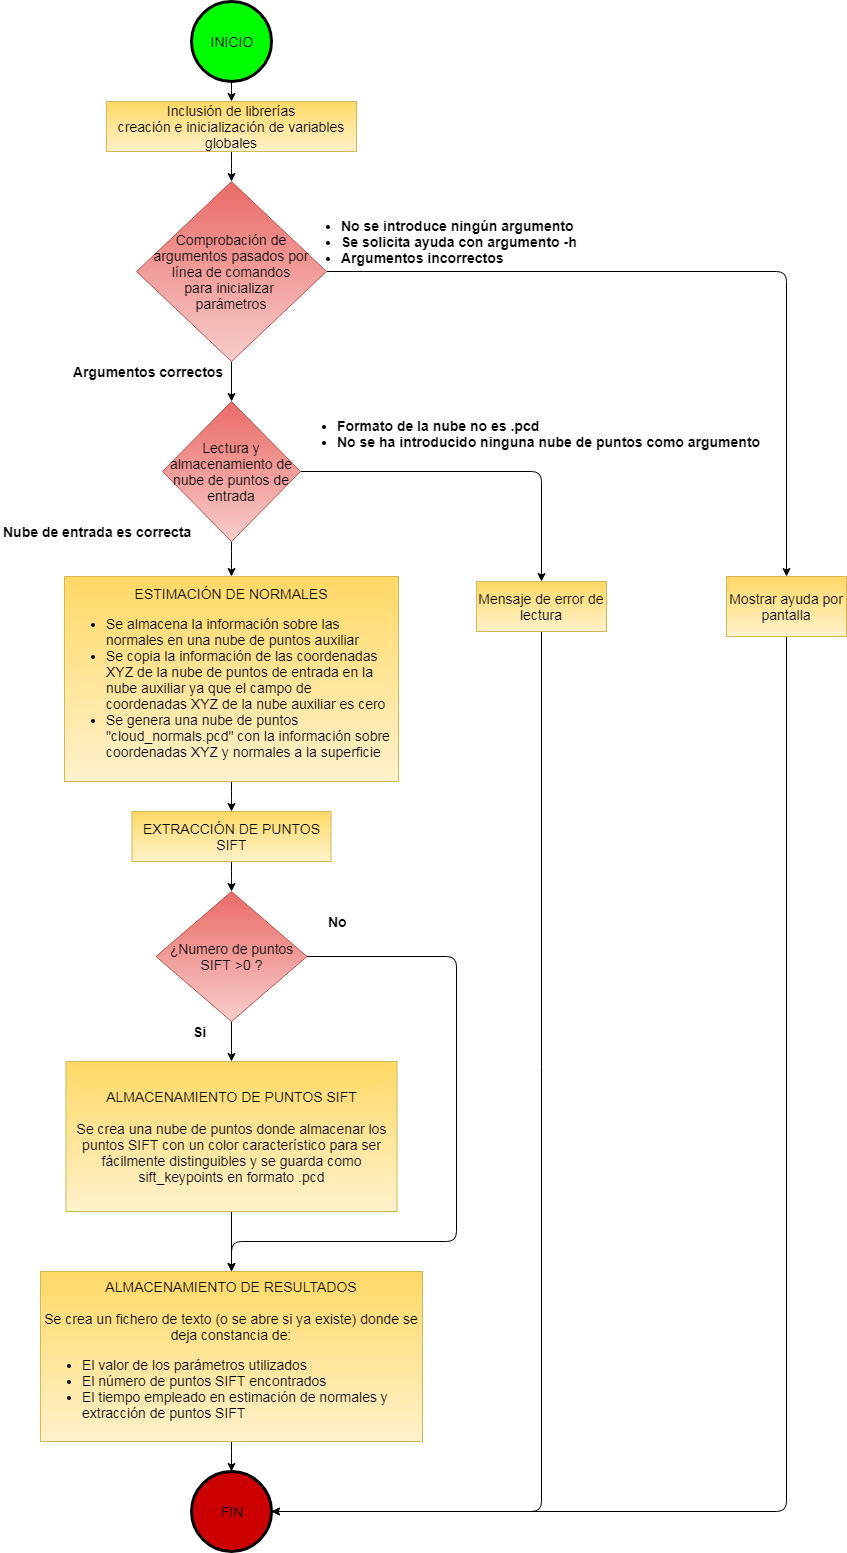
\includegraphics[scale=0.45]{main_HL_diagram}
\caption{Flujograma que representa el proceso de extracción de puntos SIFT.}\label{fig:main_HL_diagram}
\end{figure}

\subsubsection{Explicación en bajo nivel}\label{sift_bajo_nivel}
En esta ocasión se parte de un ejemplo disponible en la documentación de PCL\cite{ejemplo_narf} en el que se extraen otro tipo de keypoints, NARF en vez de SIFT. Para conseguir extraer puntos SIFT, el autor de este trabajo ha hecho uso de la documentación disponible en cuanto a la clase y métodos de C++ correspondientes\cite{sift_class} y ha procedido de forma análoga al ejemplo mencionado efectuando las modificaciones pertinentes, entre ellas, eliminando la visualización de los keypoints resultantes (de ello se encarga el programa de visualización ya visto en el apartado \ref{visualizacion}) y haciendo uso de otro tipo de parámetros necesarios para la estimación.
\\
\\
En lo que al código se refiere, tras la inclusión de las librerías necesarias, se crean e inicializan el conjunto de variables globales necesarias cuyo significado se explicará según se requiera su uso a lo largo del programa. Como excepción se tienen las variables $begin$, $end$, $elapsed\_sec$, $normal\_estimation\_time$ y $sift\_estimation\_time$ que sirven para medir tiempos de ejecución por lo que entrarán en juego en el siguiente capítulo.

\begin{lstlisting}[language=C++,breaklines]
int normal_estimation_object = 0;
float radius_search = 0.02f;
float normal_estimation_time = 0.0f;
float sift_estimation_time = 0.0f;

float min_scale = 0.01f;
int n_octaves = 3;
int n_scales_per_octave = 4;
float min_contrast = 0.001f;
int sift_points=0; 

clock_t begin,end;
double elapsed_sec;
\end{lstlisting}

\iffalse
Se implementa ahora el método que muestra ayuda por pantalla que informa sobre cómo utilizar el programa y los posibles parámetros que acepta.

\begin{lstlisting}[language=C++,breaklines]
void 
printUsage (const char* progName)
{
  std::cout << "\n\nUsage: "<<progName<<" [options] <scene.pcd>\n\n"
            << "Options:\n"
            << "-------------------------------------------\n"
            << "-o <integer>	0 for regular normal estimation (default), 1 for enhanced normal estimation\n"
            << "-r <float>	Radius search for normal estimation (default "<< radius_search<<")\n"
            << "-ms <float>	Minimum scale (default " << min_scale << ")\n"
            << "-no <int>	Number of octaves (default " << n_octaves << ")\n"
            << "-ns <int>	Number of scales per octave (default " << n_scales_per_octave << ")\n"
	    	<< "-mc <float>	Minimum contrast (default " << min_contrast << ")\n"
	    	<< "-h		Show help\n"
            << "\n\n";
}
\end{lstlisting}
\fi

A continuación, se implementa el método principal ``main'' y que ocupa el resto del código.\\
Primeramente, se comprueba si el número de argumentos es el correcto o se ha pedido ayuda con el argumento $-h$ y se muestran por pantalla el valor de los parámetros, ya sea el establecido con argumentos por línea de comandos o sus valores por defecto.
Además, se crea la instancia $ne$ de la clase $NormalEstimation$ o $NormalEstimationOMP$ según el valor del parámetro correspondiente pasado por línea de comandos. La clase $NormalEstimation$ sirve para la estimación estándar de normales mientras que $NormalEstimationOMP$ permite realizar esta misma operación entre 6 y 8 veces más rápido para equipos con procesadores de 8 núcleos (queda excluida la FPGA usada en el presente trabajo). Esta clase es compatible con la estándar pero solamente se aprecian mejoras sustanciales en tiempo de computación si se dispone de un equipo suficientemente potente.



\begin{lstlisting}[language=C++,breaklines]
int main(int argc, char** argv)
{
  if(argc == 1 || (pcl::console::find_argument (argc,argv,"-h") >= 0) )
  {
	printUsage (argv[0]);
	return 0;
  }	

  std::cout << std::endl << "---Normal estimation parameters---" << std::endl;

  pcl::NormalEstimation<pcl::PointXYZ, pcl::PointNormal> ne;
  pcl::console::parse (argc, argv, "-o", normal_estimation_object);
  if(normal_estimation_object >0)
  {
	std::cout << "Using enhanced normal estimation object" << std::endl;
	pcl::NormalEstimationOMP<pcl::PointXYZ, pcl::PointNormal> ne;
  }
  else
  {
	std::cout << "Using regular normal estimation object" << std::endl;
  }
  
  pcl::console::parse (argc,argv, "-r", radius_search);
  std::cout << "Setting radius search for normal estimation to: " << radius_search << std::endl;

  
  std::cout << std::endl << "---Sift points parameters---" << std::endl;
  
  
  pcl::console::parse (argc,argv, "-ms", min_scale);
  std::cout << "Setting minimum scale to: " << min_scale << std::endl;

  pcl::console::parse (argc,argv, "-no", n_octaves);
  std::cout << "Setting number of octaves to: " << n_octaves << std::endl;

  pcl::console::parse (argc,argv, "-ns", n_scales_per_octave);
  std::cout << "Setting number of scales per octave to: " << n_scales_per_octave << std::endl;

  pcl::console::parse (argc,argv, "-mc", min_contrast);
  std::cout << "Setting minimum contrast to: " << min_contrast << std::endl;

  std::cout << std::endl << std::endl;
\end{lstlisting}

Ahora se efectúa la lectura de la nube de puntos comprobando que se ha introducido como argumento un archivo en formato PCD y que éste puede leerse. La nube se almacena en $cloud\_xyz$ que es una instancia de la clase $PointCloud$.

\begin{lstlisting}[language=C++,breaklines]
  begin = clock();

  pcl::PointCloud<pcl::PointXYZ>::Ptr cloud_xyz (new pcl::PointCloud<pcl::PointXYZ>);
  std::vector<int> pcd_filename_indices = pcl::console::parse_file_extension_argument (argc, argv, "pcd"); 
  std::string filename;
     
  std::cout << "Reading file..." << std::endl;

  if (!pcd_filename_indices.empty ())
  {
  	filename = argv[pcd_filename_indices[0]];
  	if (pcl::io::loadPCDFile (filename, *cloud_xyz) == -1) 
    	{
        	std::cout << "Was not able to open file \""<<filename<<"\".\n";
       		return -1;
    	}
  }
  else
  {
  	std::cout << "\nNo *.pcd file given => closing.\n\n";
  	return -1;
  }
  
  end = clock();
  elapsed_sec = double(end-begin)/CLOCKS_PER_SEC;
  std::cout << "Number of points in "<< filename << ": "<< cloud_xyz->points.size () <<std::endl; 
  std::cout << "Time needed for " << filename << " to load: " << elapsed_sec << " seconds"<< std::endl << std::endl; 
\end{lstlisting}
  
  
La siguiente parte del código se encarga de la extracción de normales en la superficie de la nube\cite{normal}. Para ello se crea una instancia de la clase $PointCloud$ llamada $cloud\_normals$ y que va a almacenar una nube de puntos idéntica a la de entrada pero con información adicional sobre los vectores normales.
\\
\\
Retomando la instancia $ne$ de la clase $NormalEstimation$, se llama al método $setInputCloud$ para asignar a esta instancia la nube de puntos con la que va a trabajar, es decir, $cloud\_xyz$, para que extraiga de ella los vectores normales.
Además, entran en juego un par de parámetros que se asignan con los métodos $setSearchMethod$ y $setRadiusSearch$ y sirven para establecer respectivamente el método de búsqueda de normales y el radio de la esfera (en centímetros) dentro de la que buscar normales, siendo el centro de la misma cada punto de la nube en cada iteración. Debe cumplirse que $radius\_search>0.$
\\
\\
El método de búsqueda de normales se establece usando la instancia $tree\_n$ de la clase $KdTree$ y hace referencia a la partición o clasificación jerárquica del espacio en forma de árbol para agilizar las operaciones sobre la nube $cloud\_xyz$.
\\
\\
Una vez que todos los parámetros están asignados, se llama al método $compute$ indicando que es la nube $cloud\_normals$ en la que hay que almacenar la información de los vectores normales extraídos de $cloud\_xyz$.

\begin{lstlisting}[language=C++,breaklines]
  pcl::PointCloud<pcl::PointNormal>::Ptr cloud_normals (new 		pcl::PointCloud<pcl::PointNormal>);
  pcl::search::KdTree<pcl::PointXYZ>::Ptr tree_n(new pcl::search::KdTree<pcl::PointXYZ>());

  ne.setInputCloud(cloud_xyz);
  ne.setSearchMethod(tree_n);
  ne.setRadiusSearch(radius_search);
 
  std::cout << "Estimating normals in " << filename << " surface..." <<std::endl;

  begin = clock();
  ne.compute(*cloud_normals);
  end = clock();

  normal_estimation_time = double(end-begin)/CLOCKS_PER_SEC;
  std::cout << "Time needed for normal estimation (compute) in " << filename << ": " << normal_estimation_time << " seconds" << std::endl << std::endl;
\end{lstlisting}
  
\iffalse
Debido a que el método $compute$ solamente guarda en $cloud\_normals$ los vectores normales extraídos de la nube $cloud\_xyz$, la primera carece de información de coordenadas XYZ sobre los puntos originales. Por lo tanto, se copia dicha información de $cloud\_xyz$ a $cloud\_normals$.

\begin{lstlisting}[language=C++,breaklines]
  std::cout << "Copying xyz information from" << filename << " to cloud with normals information..." << std::endl;

  begin = clock();

  for(size_t i = 0; i<cloud_normals->points.size(); ++i)
  {
  	cloud_normals->points[i].x = cloud_xyz->points[i].x;
  	cloud_normals->points[i].y = cloud_xyz->points[i].y;
  	cloud_normals->points[i].z = cloud_xyz->points[i].z;
  }

  end = clock();
  elapsed_sec = double(end-begin)/CLOCKS_PER_SEC;
  std::cout << "Time needed for copying the pointcloud: " << elapsed_sec <<" seconds" << std::endl << std::endl;
\end{lstlisting}
\fi

  Si la nube $cloud\_normals$ no está vacía, se guarda en formato PCD bajo el nombre $cloud\_normals.pcd$
  
\begin{lstlisting}[language=C++,breaklines]
  if(cloud_normals->points.size()!=0){
  	pcl::io::savePCDFileASCII ("cloud_normals.pcd", *cloud_normals);
  }
\end{lstlisting}

El siguiente bloque de código hace referencia a la extracción de puntos SIFT creando en primer lugar la instancia $sift$ de la clase $SIFTKeypoint$, es decir, un punto del tipo SIFT sobre el cual se efectúan las operaciones pertinentes. Además, el resultado de la extracción, la nube con los puntos SIFT, se almacena en la instancia $result$ de la clase $PointCloud$.

\begin{lstlisting}[language=C++,breaklines]
  pcl::SIFTKeypoint<pcl::PointNormal, pcl::PointWithScale> sift;
  pcl::PointCloud<pcl::PointWithScale>::Ptr result(new pcl::PointCloud<pcl::PointWithScale>);
  pcl::search::KdTree<pcl::PointNormal>::Ptr tree(new pcl::search::KdTree<pcl::PointNormal> ());
  sift.setSearchMethod(tree);
  sift.setScales(min_scale, n_octaves, n_scales_per_octave);
  sift.setMinimumContrast(min_contrast);
  sift.setInputCloud(cloud_normals);
 
  std::cout << "Estimating sift points in " << filename << "..." << std::endl;

  begin = clock();
  sift.compute(*result);
  end = clock();
  sift_estimation_time = double(end-begin)/CLOCKS_PER_SEC;
  std::cout << "Time needed for sift point extraction: " << sift_estimation_time << " seconds" << std::endl << std::endl;
\end{lstlisting}


En el fragmento de código anterior entran en juego más parámetros que en la extracción de normales. Como ya se ha indicado antes, se crea una instancia $tree$ de la clase $KdTree$\cite{kdtree} para la labor de partición y organización jerárquica del espacio en forma de árbol y se asigna a $sift$ mediante el método $setSearchMethod$.
El método $setScales$ se encarga de asignar a $sift$ los parámetros $min\_scale$, $n\_octaves$ y $n\_scales\_per\_octave$ del tipo $float$, $int$ e $int$ respectivamente. Su significado es el siguiente:

\begin{itemize}
\item[•]$min\_scale$: Es la desviación estándar de la función Gaussiana para el primer desenfoque aplicado a la nube.
\item[•]$n\_octaves$: Número de octavas o conjunto de nubes del mismo tamaño a las que se les aplica diferentes desenfoques.
\item[•]$n\_scales\_per\_octave$: Es el número de desenfoques por octava.
\end{itemize}

Para comprender estos parámetros, hay que tener en cuenta que el algoritmo de extracción de puntos SIFT crea un espacio escalado a partir de la nube con la que trabaja. Esto se debe a que trata de reproducir la naturaleza ``multiescala''\cite{sift_escala} de los objetos en la realidad, es decir, los detalles que se aprecian de un árbol, por ejemplo, varían según la distancia a la que se encuentra el observador: a cincuenta metros de distancia se precia la forma, tamaño y colores principales del árbol mientras que a un metro de distancia se pueden ver otros detalles como la rugosidad del tronco o forma de las hojas. Además, dependiendo del observador, el nivel de los detalles detectados en el árbol varían.
\\
\\
Considerando una nube de puntos en dos dimensiones como una imagen plana, para construir un espacio escalado en primer lugar se toma la nube de puntos original con la función que la describe: 
$$f(x,y)$$ 
\\
junto a la función Gaussiana:
$$G(x,y,\sigma)=\frac{1}{2\pi\sigma^2}e^{-\frac{x^2+y^2}{2\sigma^2}}$$
\\
y se difumina, es decir, se hace una convolución\cite{gaussiana} 
$$L(\cdot,\cdot,\sigma)=G(\cdot,\cdot,\sigma)*f(\cdot,\cdot)$$
\\
La convolución se aplica para cada valor $x$ e $y$ siendo así el parámetro principal de la función Gaussiana la desviación típica $\sigma$ que se indica con $min\_scale$. Esta operación se repite un número de veces indicado por el parámetro $n\_scales\_per\_octave$ e incrementando en cada iteración el valor de la desviación típica y por tanto el nivel de desenfoque.
\\
Cuando se alcanza el número máximo de iteraciones, se toma la nube a la que se le ha aplicado el desenfoque con el mayor valor de la desviación típica y se reduce su tamaño a la mitad. Una vez hecho esto, se repite el proceso anterior para difuminar la nube mediante la función Gaussiana e incrementando su valor de la desviación típica. 
\\
\\
El proceso de reducción del tamaño de la nube para aplicar la convolución con la función Gaussiana se repite un número de veces indicado por el parámetro $n\_octaves$, es decir, número de octavas, ya que el tamaño de la nube se reduce a la mitad.
\\
\\
El proceso de creación del espacio escalado se puede visualizar en el ejemplo de la figura \ref{fig:filtro_gauss}. El propósito de este conjunto de operaciones es el de simular diferentes escalas de observación (movimiento vertical en la figura \ref{fig:filtro_gauss}) así como la apreciación de diferentes niveles de detalle en cada escala (movimiento horizontal en la figura \ref{fig:filtro_gauss})  
\\
\\
\begin{figure}
\centering
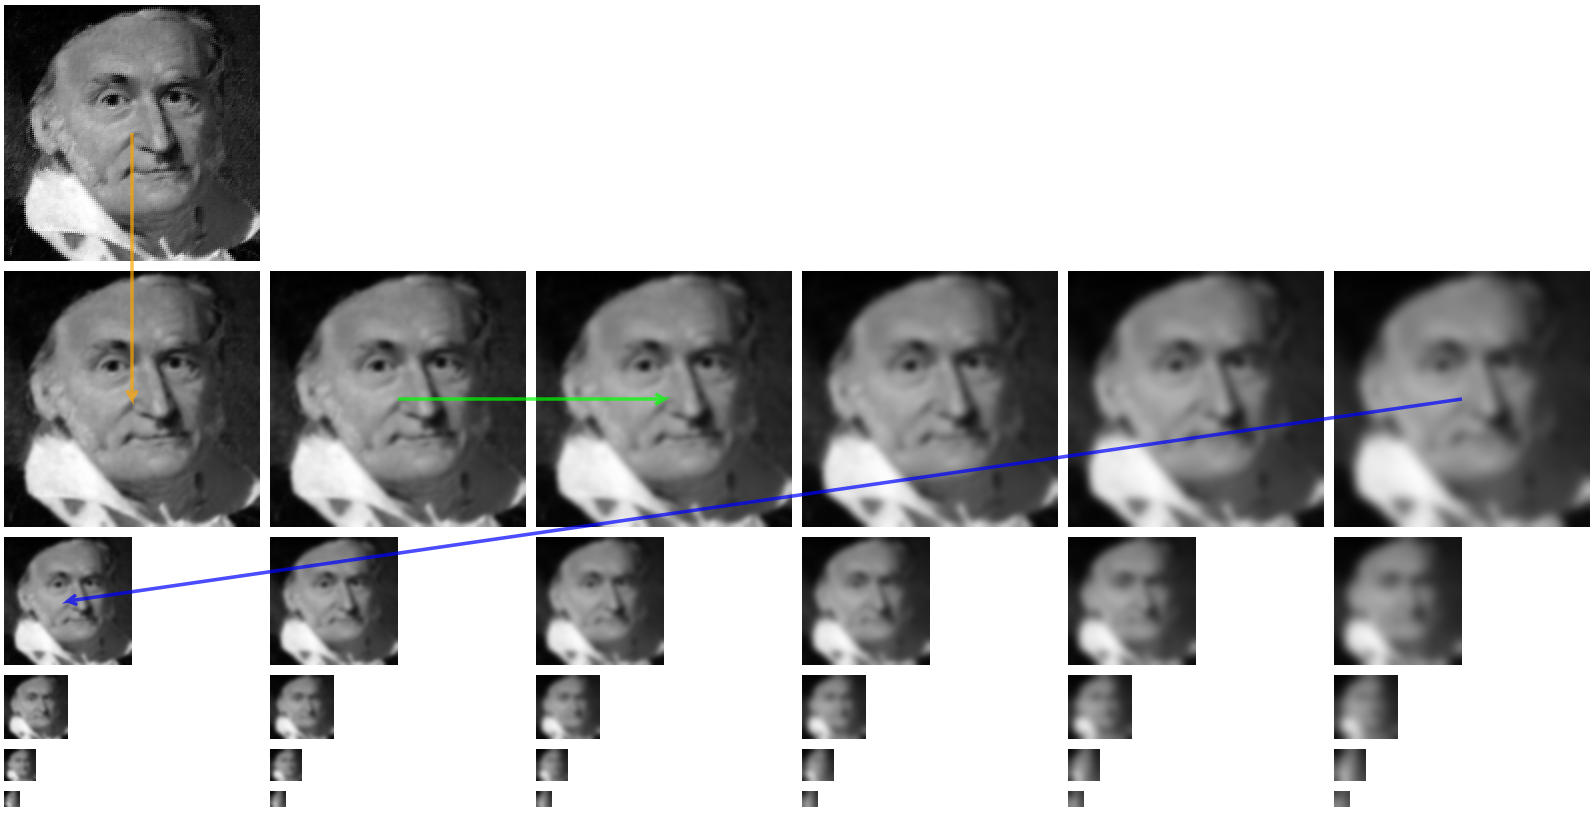
\includegraphics[scale=0.42]{filtro_gauss}
\caption{Ejemplo de creación de un espacio escalado. La flecha naranja indica el primer desenfoque aplicado a la imagen original. La flecha verde indica la convolución de la imagen con la función Gaussiana para desviaciones típicas crecientes. La flecha azul indica la creación de una nueva octava.}\label{fig:filtro_gauss}
\end{figure}
%https://en.wikipedia.org/wiki/Scale_space
%http://aishack.in/tutorials/sift-scale-invariant-feature-transform-scale-space/
%http://weitz.de/sift/
%http://aishack.in/tutorials/harris-corner-detector/
El último parámetro es $min\_contrast$ y se asigna a $sift$ con $setMinimumContrast$. Este parámetro actúa como un filtro para eliminar los puntos SIFT que no tienen suficiente contraste. Esto se consigue calculando dos gradientes perpendiculares en cada keypoint detectado de forma que la superficie entorno al keypoint puede ser plana (ambos gradientes tienen un valor pequeño), representar un borde (un gradiente tiene un valor elevado y el otro no) o representar una esquina (ambos gradientes toman valores significativos). Poner este parámetro a cero significa aceptar todos los keypoints detectados mientras que incrementarlo aumenta la dureza de la criba y por tanto la exigencia de contraste en cada uno de ellos.
\\
\\
Con $setInputCloud$ se asigna a $sift$ la nube con la que se trabaja que en el caso es $cloud\_normals$ y con $compute$ se efectúa la operación de extracción de puntos SIFT para almacenarlos en $result$.
\\
%http://aishack.in/tutorials/harris-corner-detector/
Si la nube $result$ no está vacía, es decir, se han encontrado puntos SIFT, se crea una instancia de una nueva nube llamada $keypoints$ y en ella se almacenan los puntos SIFT encontrados con información adicional sobre su color pues ahora serán verdes para su fácil visualización. Después, se guarda la nube $keypoints$ en formato PCD bajo el nombre $sift\_keypoints.pcd$. Esta nube de puntos junto a la nube de la que procede y de la cual se han extraído los keypoints, son las que se utilizan en el visualizador para apreciar una nube de puntos con sus keypoints resaltados.
\\
\\
\iffalse
\begin{lstlisting}[language=C++,breaklines]
  if(result->points.size()>0){
  
  	std::cout << "Number of SIFT points in " << filename << ": " << result->points.size () << std::endl;

	sift_points = result->points.size();

	pcl::PointCloud<pcl::PointXYZRGBA>::Ptr keypoints(new pcl::PointCloud<pcl::PointXYZRGBA>);
  
	keypoints->width = result->width;
	keypoints->height = result->height;
	keypoints->points.resize(keypoints->width * keypoints->height);

   	for (size_t i = 0; i < result->points.size (); ++i)
  	{
    	keypoints->points[i].x = result->points[i].x;
    	keypoints->points[i].y = result->points[i].y;
    	keypoints->points[i].z = result->points[i].z;

  		keypoints->points[i].r=50;
  		keypoints->points[i].g=255;
  		keypoints->points[i].b=50;
  		keypoints->points[i].a=255;
  	}
  	pcl::io::savePCDFileASCII ("sift_keypoints.pcd", *keypoints);
  }
  else {
  	std::cout << "No sift points found" << std::endl;
	sift_points = 0;
  }
\end{lstlisting}
\fi
Por último, a efectos de registrar resultados, se abre o crea un fichero de texto llamado $tests.txt$ en el que se indica el nombre de la nube de puntos de entrada y el número de puntos que contiene, el valor de los parámetros utilizados en todas las operaciones que los requieren y el número de puntos SIFT encontrados.
\\
\iffalse
\begin{lstlisting}[language=C++,breaklines]
  std::fstream fs;
  fs.open("tests.txt", std::fstream::app);
  
  fs << "filename: " << filename << std::endl;
  
  fs << std::endl <<  "Normal estimation radius search: " << radius_search << std::endl; 
  fs << "Minimum scale: " << min_scale << std::endl;
  fs << "Number of octaves: " << n_octaves << std::endl;
  fs << "Number of scales per octave: " << n_scales_per_octave << std::endl;
  fs << "Minimum contrast: " << min_contrast << std::endl;

  fs << std::endl << "Normal estimation time (s): " << normal_estimation_time << std::endl;
  fs << "SIFT points estimation time (s): " << sift_estimation_time << std::endl;
  fs << "Number of SIFT points found: " << sift_points << std::endl;

  fs << "---------------------\n----------------------\n";
  fs.close();
  return 0;
}
\end{lstlisting}
\fi
No se muestra el código de estas últimas operaciones ya que es trivial pues solamente se guardan resultados en ficheros de texto y variables.

\section{Ejemplos}
Los siguientes ejemplos se han llevado a cabo en una computadora que dispone de máquina virtual con sistema operativo basado en linux. Todos ellos son reproducibles en el sistema embebido salvo los de visualización como ya se ha indicado previamente.

Se van a tomar como ejemplos tres nubes de puntos:
\begin{itemize}
\item[•]$bunny.pcd$: 
Con un total de 397 puntos representa un conejo. El encabezamiento del archivo es el siguiente:\\
\begin{lstlisting}
#bunny.pcd
#.PCD v.5 - Point Cloud Data file format
VERSION .5
FIELDS x y z
SIZE 4 4 4
TYPE F F F
COUNT 1 1 1
WIDTH 397
HEIGHT 1
POINTS 397
DATA ascii
\end{lstlisting}

\item[•]$cturtle.pcd$:
Contiene 167198 puntos que representan el caparazón de una tortuga en forma de nube desordenada, es decir, su estructura es vectorial ya que su atributo HEIGHT es la unidad y WIDTH toma como valor la totalidad de los puntos de la nube. El encabezamiento del archivo se muestra a continuación:\\
\begin{lstlisting}
#cturtle.pcd
#.PCD v0.7 - Point Cloud Data file format
VERSION 0.7
FIELDS x y z intensity
SIZE 4 4 4 4
TYPE F F F F
COUNT 1 1 1 1
WIDTH 167198
HEIGHT 1
VIEWPOINT 0 0 0 1 0 0 0
POINTS 167198
DATA binary_compressed
\end{lstlisting}


\item[•]$milk\_cartoon\_all\_small\_clorox.pcd$:
Representa tres botes sobre una superficie mediante 307200 puntos. Su encabezamiento indica que es una nube ordenada, es decir, tiene una estructura matricial tal y como se indicó en la explicación del formato PCD.\\
\begin{lstlisting}
#milk_cartoon_all_small_clorox.pcd
#.PCD v0.7 - Point Cloud Data file format
VERSION 0.7
FIELDS x y z rgba
SIZE 4 4 4 4
TYPE F F F U
COUNT 1 1 1 1
WIDTH 640
HEIGHT 480
VIEWPOINT 0 0 0 1 0 0 0
POINTS 307200
DATA binary_compressed
\end{lstlisting}

\end{itemize}

Se puede apreciar en los encabezamientos de las nubes que el tipo de datos en $bunny.pcd$ es $ASCII$ mientras que en las otras dos nubes es $binary\_compressed$. Esto se debe a la gran cantidad de puntos que contienen por lo que el formato $ascii$ se comprime en $binary\_compressed$ para que el archivo ocupe menos espacio.

\subsection{Visualización de nubes}
Para visualizar estas nubes se ejecutan los siguientes comandos pudiendo ver los resultados en las figuras \ref{fig:bunny_ejemplo}, \ref{fig:cturtle_ejemplo} y \ref{fig:botes} 
$$./visualization\;\;bunny.pcd$$
$$./visualization\;\;cturtle.pcd$$
$$./visualization\;\;milk\_cartoon\_all\_small\_clorox.pcd$$

\begin{figure}[!htb]
\minipage{0.32\textwidth}
  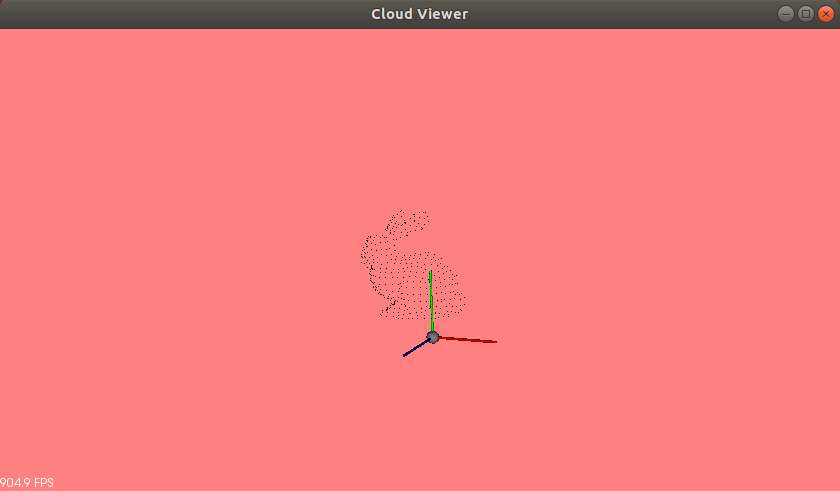
\includegraphics[width=\linewidth]{bunny_ejemplo}
  \caption{Visualización de la nube $bunny.pcd$}\label{fig:bunny_ejemplo}
\endminipage\hfill
\minipage{0.32\textwidth}
  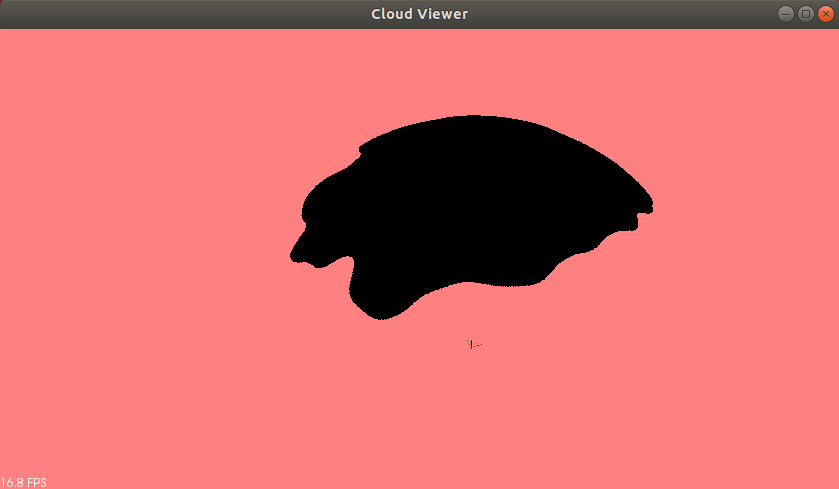
\includegraphics[width=\linewidth]{cturtle_ejemplo}
  \caption{Visualización de la nube $cturtle.pcd$}\label{fig:cturtle_ejemplo}
\endminipage\hfill
\minipage{0.33\textwidth}
  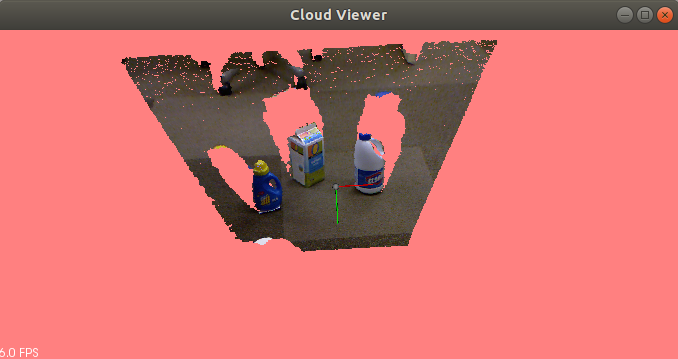
\includegraphics[width=\linewidth]{botes}
  \caption{Visualización de la nube $milk\_cartoon\_all\_small\_clorox.pcd$}\label{fig:botes}
\endminipage\hfill
\end{figure}

\subsection{Extracción de puntos SIFT}

Para hacer uso del programa $sift\_keypoints$ hay que tener en cuenta que necesita ciertos argumentos: parámetros y nube de puntos. Los primeros son opcionales ya que tienen valores por defecto pero el segundo es obligatorio. La forma de pasar parámetros va por parejas, se indica en primer lugar el nombre del parámetro y a continuación su valor:

$$-parametro1 \;\; valor1 \;\; -parametro2 \;\; valor2 \;\; ... \;\; -parametroN \;\; valorN \;\; nube.pcd$$
\\
La lista de parámetros que acepta el programa y las variables internas a las que se refieren (ya explicadas en el apartado \ref{sift_bajo_nivel}) es la siguiente:
\begin{itemize}
\item[•]\textbf{-r:} $radius\_search$, por defecto 0.02
\item[•]\textbf{-ms:} $min\_scale$, por defecto 0.01
\item[•]\textbf{-no:} $n\_octaves$, por defecto 3
\item[•]\textbf{-ns:} $n\_scales\_per\_octave$, por defecto 4
\item[•]\textbf{-mc:} $min\_contrast$, por defecto 0.001
\item[•]\textbf{-h:} help, muestra ayuda por pantalla
\end{itemize}
Además, para ejecutar este programa, se requieren permisos de super usuario debido a operaciones de escritura tal y como son modificar y guardar un fichero de texto o guardar nubes de puntos en formato PCD.
\\
\\
Ahora se quieren extraer los puntos SIFT de estas nubes por lo que se ejecutan los siguientes comandos.
$$./sift\_keypoints\;\;bunny.pcd$$
$$./sift\_keypoints\;\;cturtle.pcd\;\;-mc\;\;0$$
$$./sift\_keypoints\;\;milk\_cartoon\_all\_small\_clorox.pcd$$
\\
\\
Se han utilizado el valor de los parámetros por defecto en $bunny.pcd$ y \\
$milk\_cartoon\_all\_small\_clorox.pcd$ pero no ha sido así en $cturtle.pcd$ ya que el parámetro $minimum\_contrast$ tiene un valor de $0$ en vez de $0,001$. Esto se debe a que ninguno de los puntos SIFT detectados supera el filtro de contraste, lo cual parece razonable porque estudiando la superficie que representa $cturtle.pcd$ se ve una curvatura muy suave y a penas tiene bordes y esquinas marcados.
\\
\\
De este modo, el fichero de texto $tests.txt$ generado tras ejecutar estos tres comandos tiene el siguiente contenido:

\begin{lstlisting}
filename: bunny.pcd

Normal estimation radius search: 0.02
Minimum scale: 0.01
Number of octaves: 3
Number of scales per octave: 4
Minimum contrast: 0.001

Normal estimation time (s): 0.034731
SIFT points estimation time (s): 0.040729
Number of SIFT points found: 13
------------------------------
------------------------------
filename: milk_cartoon_all_small_clorox.pcd

Normal estimation radius search: 0.02
Minimum scale: 0.01
Number of octaves: 3
Number of scales per octave: 4
Minimum contrast: 0.001

Normal estimation time (s): 122.083
SIFT points estimation time (s): 5.09761
Number of SIFT points found: 404
------------------------------
------------------------------
filename: cturtle.pcd

Normal estimation radius search: 0.02
Minimum scale: 0.01
Number of octaves: 3
Number of scales per octave: 4
Minimum contrast: 0

Normal estimation time (s): 14.1584
SIFT points estimation time (s): 9.5875
Number of SIFT points found: 952
\end{lstlisting}

Además, cada vez que se extraen los puntos SIFT de una nube, se genera una nube de puntos llamada $sift\_keypoints$ la cual contiene los puntos SIFT de la nube de entrada a este programa. Esto es importante de cara a la siguiente sección de visualización de puntos SIFT.


\subsection{Visualización de puntos SIFT}
Por último, se visualizan en conjunto la nube original y sus puntos SIFT utilizando de nuevo el visualizador el cual se alimenta de dos nubes de puntos: la nube original y la nube $sift\_keypoints$ que contiene sus puntos SIFT y ha sido generada por el programa de extracción de keypoints. En las figuras \ref{fig:botes_ejemplo_sift}, \ref{fig:bunny_ejemplo_sift} y \ref{fig:cturtle_ejemplo_sift} se aprecian los resultados de ejecutar los siguientes comandos:

$$./visualization\;\;bunny.pcd\;\;sift\_keypoints.pcd$$
$$./visualization\;\;milk\_cartoon\_all\_small\_clorox.pcd\;\;sift\_keypoints.pcd$$
$$./visualization\;\;cturtle.pcd\;\;sift\_keypoints.pcd$$


\begin{figure}[!htb]
\minipage{0.32\textwidth}
  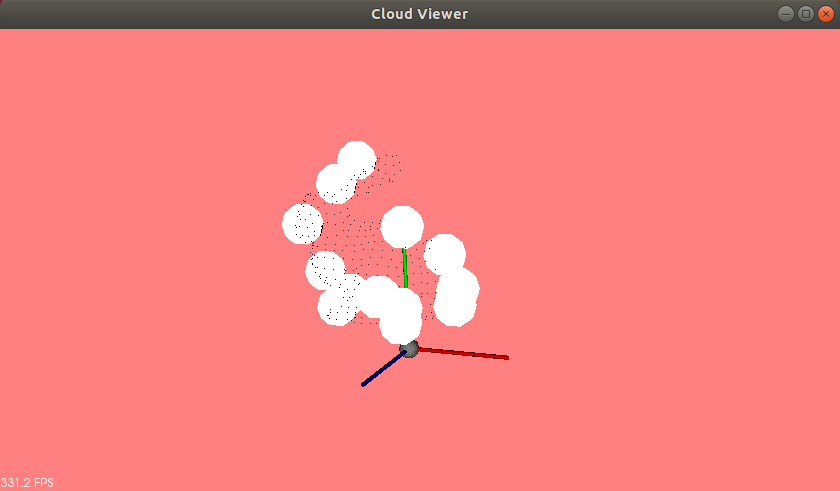
\includegraphics[width=\linewidth]{bunny_ejemplo_sift}
  \caption{Visualización de la nube $bunny.pcd$ junto a sus puntos SIFT como esferas blancas.}\label{fig:bunny_ejemplo_sift}
\endminipage\hfill
\minipage{0.32\textwidth}
  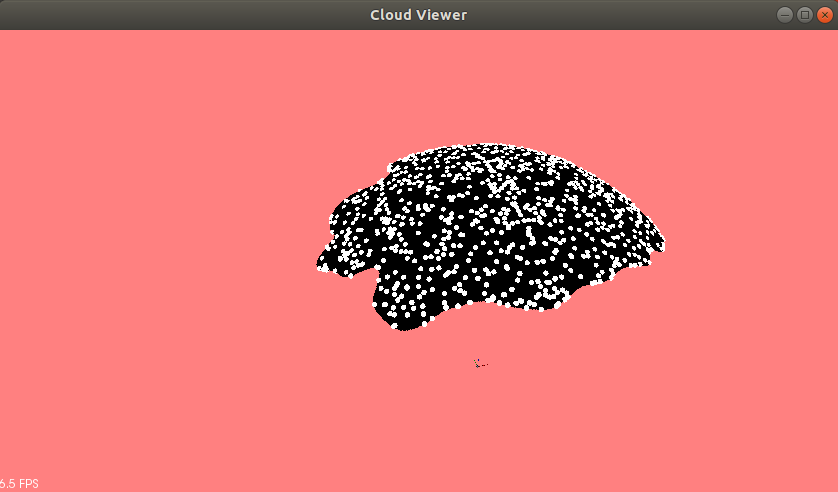
\includegraphics[width=\linewidth]{cturtle_ejemplo_sift}
  \caption{Visualización de la nube $cturtle.pcd$ junto a sus puntos SIFT como esferas blancas.}\label{fig:cturtle_ejemplo_sift}
\endminipage\hfill
\minipage{0.33\textwidth}
  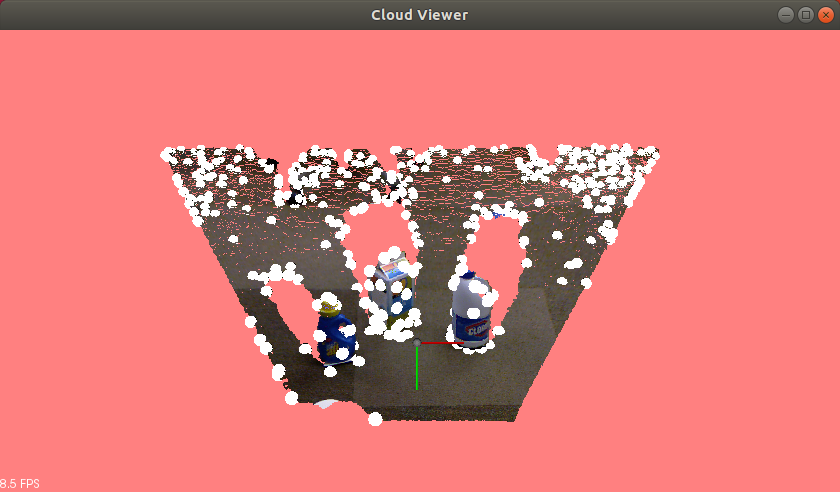
\includegraphics[width=\linewidth]{botes_ejemplo_sift}
  \caption{Visualización de la nube $milk\_cartoon\_all\_small\_clorox.pcd$ junto a sus puntos SIFT como esferas blancas.}\label{fig:botes_ejemplo_sift}
\endminipage\hfill
\end{figure}


\section{Conclusiones}
Se ha visto en este capítulo cómo el autor ha creado un pipeline completo de visualización de nubes de puntos y extracción de puntos SIFT a partir de la documentación de PCL. Además se ha mostrado su uso en tres nubes de puntos de diferentes características.
\\
En el siguiente capítulo se procederá a medir los tiempos de ejecución de los algoritmos de estimación de vectores normales y puntos SIFT para determinar cuál es el de mayor carga computacional.

\chapter{Medición de tiempos de ejecución}

\section{Introducción}
Se ha mencionado en el capítulo anterior que el programa de extracción de puntos SIFT, $sift\_keypoints$, consta de dos partes principales entre otras como pueden ser cargar librerías, crear o modificar ficheros de texto o copiar información de una nube de puntos a otra. Estas dos partes son la extracción de vectores normales a la superficie descrita por la nube de puntos con la que trabaja el programa y la estimación de puntos SIFT.


En este capítulo se va a presentar una forma sencilla de medir los tiempos de ejecución de estos dos procesos a la vez que se modifican los parámetros que influyen en ellos. De este modo, se determinará si será la estimación de normales o la de puntos SIFT la parte necesita ser llevada a hardware digital para su posterior optimización. Estas pruebas se van a realizar sobre la FPGA puesto que es en este hardware donde se desarrollarán los objetivos principales del TFG.

Además, se ha creado una sección exclusiva para los gráficos dada la gran cantidad de ellos que hay.


\section{Método de medición}
Trabajando en C++, como de costumbre, el proceso de medición de tiempos requiere la inclusión de la librería $ctime$ para lo cual se tiene al comienzo del código en $sift\_keypoints.cpp$.

\begin{lstlisting}[language=C++,breaklines]
	#include <ctime>
\end{lstlisting}

Incluída esta librería, ahora se pueden utilizar las variables globales $begin$,$end$ y $elapsed\_sec$ declaradas de la siguiente manera:

\begin{lstlisting}[language=C++,breaklines]
	clock_t begin,end;
	double elapsed_sec;
\end{lstlisting}

Las variables $begin$ y $end$ son del tipo $clock\_t$ y sirven para almacenar cuentas de $clock\;\; ticks$ o ciclos de reloj mientras que $elapsed\_sec$ es del tipo double para almacenar el tiempo en segundos que ha llevado efectuar una determinada operación.\\
El proceso de medición de tiempo es el siguiente: 

\begin{lstlisting}[language=C++,breaklines]
	begin = clock();
	process();
	end = clock();
	
	elapsed_sec = double(end - begin)/CLOCKS_PER_SEC;
\end{lstlisting}

En primer lugar se almacena en $begin$ el valor devuelto por la función $clock()$, es decir, número de ciclos de reloj que han transcurrido en el procesador desde el inicio del programa hasta su llamada. A continuación se ejecuta el proceso cuyo tiempo de ejecución desea medirse, para este ejemplo, $process()$. Ahora se actúa de manera similar al primer paso ya que se almacena en $end$ el número de ciclos transcurridos desde el inicio del programa hasta la llamada a $clock()$ después de haberse ejecutado $process()$. Por último, se toma la diferencia de ciclos entre $end$ y $begin$ para saber cuántos ciclos ha tomado la ejecución de $process()$. Sin embargo esto no es una medida directa de tiempo por lo que el número de ciclos de ejecución del proceso se divide entre una constante, el número de ciclos que duran un segundo y que se llama $CLOCKS\_PER\_SEC$. El resultado se almacena en $elapsed\_sec$ como el tiempo en segundos que ha durado la ejecución de $process()$.


\section{Resultados de medición sobre la FPGA}
Una vez visto cómo se mide el tiempo de ejecución de cualquier parte del programa $sift\_keypoints$, se rescata parte del código del mismo para indicar qué procesos van a ser sometidos a esta medición.


En la parte de estimación de normales se analiza el método $compute$ el cual realiza todas las operaciones pertinentes para almacenar en $cloud\_normals$ los vectores normales a partir de $cloud\_xyz$:


\begin{lstlisting}[language=C++,breaklines]
  pcl::PointCloud<pcl::PointNormal>::Ptr cloud_normals (new 		pcl::PointCloud<pcl::PointNormal>);
  pcl::search::KdTree<pcl::PointXYZ>::Ptr tree_n(new pcl::search::KdTree<pcl::PointXYZ>());

  ne.setInputCloud(cloud_xyz);
  ne.setSearchMethod(tree_n);
  ne.setRadiusSearch(radius_search);
 
  std::cout << "Estimating normals in " << filename << " surface..." <<std::endl;

  begin = clock();
  ne.compute(*cloud_normals);
  end = clock();

  normal_estimation_time = double(end-begin)/CLOCKS_PER_SEC;
  std::cout << "Time needed for normal estimation (compute) in " << filename << ": " << normal_estimation_time << " seconds" << std::endl << std::endl;
\end{lstlisting}

Se procede de forma análoga en la parte de estimación de puntos SIFT puesto que, tras establecer el valor de los parámetros también se llama a un método $compute$ para efectuar la extracción de keypoints:

\begin{lstlisting}[language=C++,breaklines]
  pcl::SIFTKeypoint<pcl::PointNormal, pcl::PointWithScale> sift;
  pcl::PointCloud<pcl::PointWithScale>::Ptr result(new pcl::PointCloud<pcl::PointWithScale>);
  pcl::search::KdTree<pcl::PointNormal>::Ptr tree(new pcl::search::KdTree<pcl::PointNormal> ());
  sift.setSearchMethod(tree);
  sift.setScales(min_scale, n_octaves, n_scales_per_octave);
  sift.setMinimumContrast(min_contrast);
  sift.setInputCloud(cloud_normals);
 
  std::cout << "Estimating sift points in " << filename << "..." << std::endl;

  begin = clock();
  sift.compute(*result);
  end = clock();
  sift_estimation_time = double(end-begin)/CLOCKS_PER_SEC;
  std::cout << "Time needed for sift point extraction: " << sift_estimation_time << " seconds" << std::endl << std::endl;
\end{lstlisting}

Los tiempos de ejecución del método $compute$ se almacenan en $normal\_estimation\_time$ y $sift\_estimation\_time$ para la parte de estimación de normales y puntos SIFT, respectivamente.
\\
Para aportar mayor amplitud a los resultados obtenidos, se van a realizar mediciones de los métodos $compute$ variando ligeramente los parámetros involucrados en la estimación de normales y puntos SIFT. Como se ha visto en los fragmentos de código mostrados, la extracción de normales varía con un único parámetro, $radius\_search$, mientras que el tiempo de estimación de keypoints varía con $min\_scale$, $n\_octaves$ y $n\_scales\_per\_octave$. El parámetro $min\_contrast$ no afecta al tiempo del proceso estudiado porque, como se ha visto anteriormente, indica la dureza de la criba de los puntos SIFT ya obtenidos.

Las nubes sobre las que se han realizado las pruebas son las mismas que las mostradas en el capítulo anterior: $bunny.pc$, $cturtle.pcd$ y $milk\_cartoon\_all\_small\_clorox.pcd$

Tras efectuar la medición de tiempos junto a la variación de parámetros, éstos se han plasmado en diferentes gráficas. En primer lugar, se analizan los tiempos de estimación de normales y puntos SIFT variando el parámetro $radius\_search$ puesto que la extracción de normales es la primera operación y afecta a las que vienen después. El resultado se aprecia en las figuras \ref{fig:grafico_radius_bunny}, \ref{fig:grafico_radius_cturtle} y \ref{fig:grafico_radius_milk} las cuales indican que en todos los casos un incremento del radio de búsqueda de normales a la superficie dispara el tiempo de computación mientras que el tiempo de extracción de puntos SIFT se mantiene entorno a un valor estable a pesar de que la cantidad de normales extraídas afecta a la estimación de keypoints. Resulta obvio este incremento del tiempo de computación ya que la información que hay que utilizar para estimar un vector normal se incrementa, es decir, se considera una porción de la superficie de la nube cada vez más grande.



Se muestra en las figuras \ref{fig:grafico_min_scale_bunny}, \ref{fig:grafico_min_scale_cturtle} y \ref{fig:grafico_min_scale_milk} cómo varían estos mismos tiempos modificando el parámetro $min\_scale$. Se tiene en esta ocasión algo más de variedad en los resultados obtenidos ya que en $cturtle.pcd$ y $bunny.pcd$ el tiempo de estimación de keypoints comienza siendo mayor que el de extracción de normales pero a medida que incrementa $min\_scale$ éste decrece considerablemente. Esto se debe a que la nube de entrada se convoluciona con un filtro Gaussiano cada vez más severo, es decir, un aumento de la desviación típica difumina en mayor medida la nube y hace que ésta pierda detalles finos por lo que los puntos SIFT se encuentran en esquinas o bordes muy marcados y nítidos que son capaces de persistir ante el filtro aplicado. Por otra parte, el tiempo de estimación de normales no varía ya que su único parámetro, $radius\_search$, a partir de ahora tomará el valor por defecto. En cuanto a nubes a nubes con mayor nivel de detalle y cantidad de información como en $milk\_cartoon\_all\_small\_clorox.pcd$, se puede ver que aumentar el parámetro $min\_scale$ disminuye el tiempo de estimación de puntos SIFT siendo éste ya notablemente menor que el de extracción de normales.




Ahora se modifica el parámetro $n\_octaves$ y se aprecia que para casos realistas (nubes que contienen una gran cantidad de puntos como las nubes $milk\_cartoon\_all\_small\_clorox.pcd$ y $cturtle.pcd$) como se indican en las figuras \ref{fig:grafico_n_octaves_cturtle} y \ref{fig:grafico_n_octaves_milk} el tiempo de estimación de normales es en todo caso superior al de extracción de puntos SIFT incluso aunque se afine esta búsqueda aportando  más octavas en las que estimar keypoints. No es así en una nube pequeña como $bunny.pcd$ lo cual se puede considerar un caso particular tal y como indica la figura \ref{fig:grafico_n_octaves_bunny}.



Por último, se estudia el tiempo de estimación de keypoints ante la variación del parámetro $n\_scales\_per\_octave$ apreciándose los resultados en las figuras \ref{fig:grafico_n_scales_bunny}, \ref{fig:grafico_n_scales_cturtle} y \ref{fig:grafico_n_scales_milk}. Se tiene de nuevo un tiempo de estimación de normales predominante ante la extracción de puntos SIFT para nubes con una cantidad considerable de puntos como $cturtle.pcd$ y $milk\_cartoon\_all\_small\_clorox.pcd$. En esta ocasión, incrementar el número de convoluciones de la nube por octava implica realizar más operaciones y tener en cuenta la misma nube bajo más filtros para extraer keypoints por lo que el tiempo implicado en este proceso aumenta.


\section{Resultados gráficos}

\begin{figure}[h!]
\centering
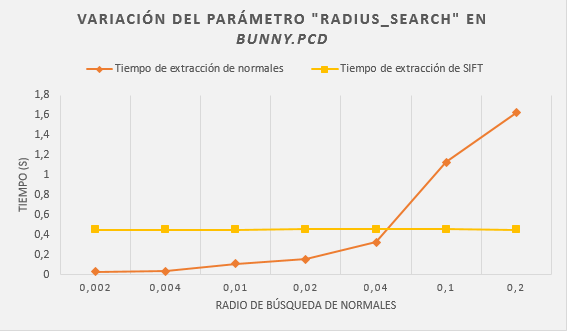
\includegraphics[scale=1]{grafico_radius_bunny}
\caption{Tiempos de estimación de normales y puntos SIFT en $bunny.pcd$ variando $radius\_search$.}\label{fig:grafico_radius_bunny}
\end{figure}

\begin{figure}[h!]
\centering
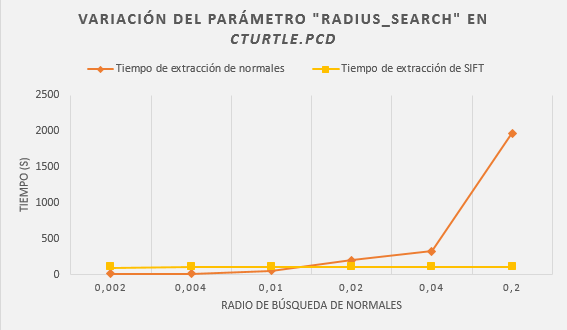
\includegraphics[scale=1]{grafico_radius_cturtle}
\caption{Tiempos de estimación de normales y puntos SIFT en $cturtle.pcd$ variando $radius\_search$.}\label{fig:grafico_radius_cturtle}
\end{figure}


\begin{figure}[h!]
\centering
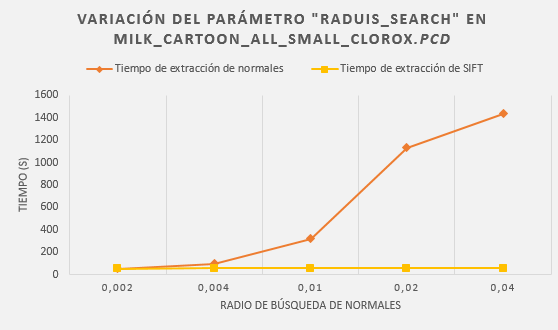
\includegraphics[scale=1]{grafico_radius_milk}
\caption{Tiempos de estimación de normales y puntos SIFT en $milk\_cartoon\_all\_small\_clorox.pcd$ variando $radius\_search$.}\label{fig:grafico_radius_milk}
\end{figure}


\begin{figure}[h!]
\centering
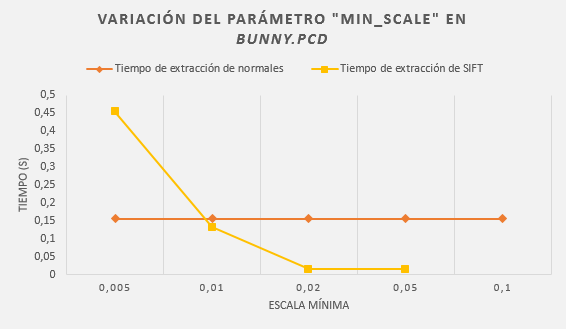
\includegraphics[scale=1]{grafico_min_scale_bunny}
\caption{Tiempos de estimación de normales y puntos SIFT en $bunny.pcd$ variando $min\_scale$.}\label{fig:grafico_min_scale_bunny}
\end{figure}

\begin{figure}[h!]
\centering
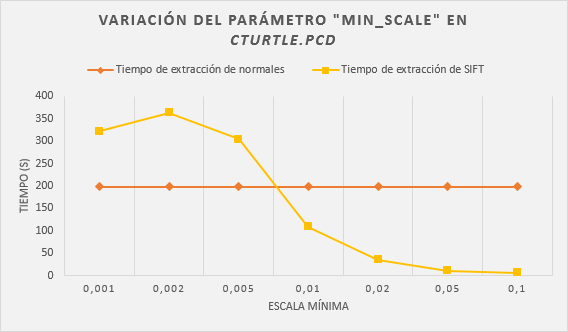
\includegraphics[scale=1]{grafico_min_scale_cturtle}
\caption{Tiempos de estimación de normales y puntos SIFT en $cturtle.pcd$ variando $min\_scale$.}\label{fig:grafico_min_scale_cturtle}
\end{figure}


\begin{figure}[h!]
\centering
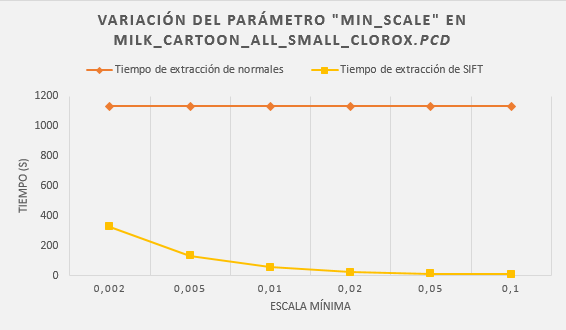
\includegraphics[scale=1]{grafico_min_scale_milk}
\caption{Tiempos de estimación de normales y puntos SIFT en $milk\_cartoon\_all\_small\_clorox.pcd$ variando $min\_scale$.}\label{fig:grafico_min_scale_milk}
\end{figure}


\begin{figure}[h!]
\centering
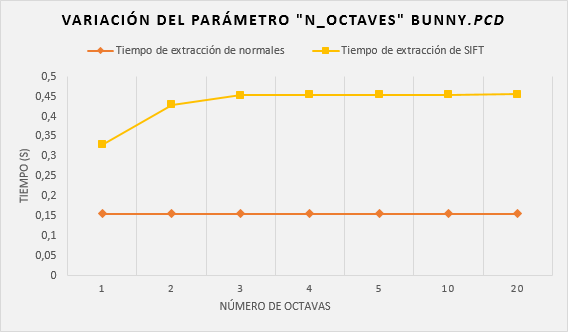
\includegraphics[scale=1]{grafico_n_octaves_bunny}
\caption{Tiempos de estimación de normales y puntos SIFT en $bunny.pcd$ variando $n\_octaves$.}\label{fig:grafico_n_octaves_bunny}
\end{figure}

\begin{figure}[h!]
\centering
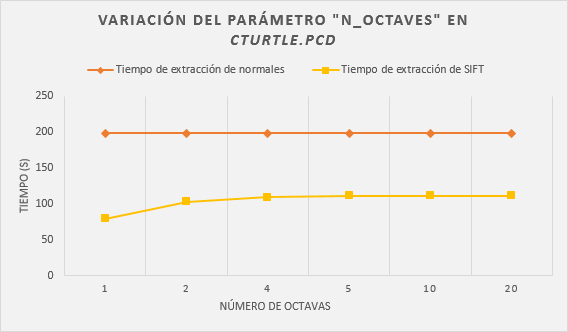
\includegraphics[scale=1]{grafico_n_octaves_cturtle}
\caption{Tiempos de estimación de normales y puntos SIFT en $cturtle.pcd$ variando $n\_octaves$.}\label{fig:grafico_n_octaves_cturtle}
\end{figure}

\begin{figure}[h!]
\centering
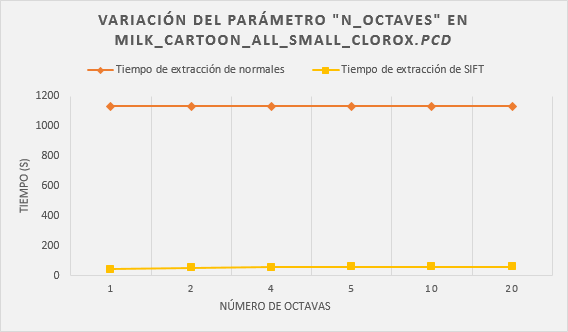
\includegraphics[scale=1]{grafico_n_octaves_milk}
\caption{Tiempos de estimación de normales y puntos SIFT en $milk\_cartoon\_all\_small\_clorox.pcd$ variando $n\_octaves$.}\label{fig:grafico_n_octaves_milk}
\end{figure}


\begin{figure}[h!]
\centering
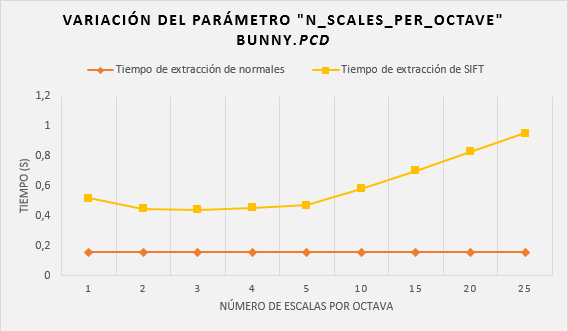
\includegraphics[scale=1]{grafico_n_scales_bunny}
\caption{Tiempos de estimación de normales y puntos SIFT en $bunny.pcd$ variando $n\_scales\_per\_octave$.}\label{fig:grafico_n_scales_bunny}
\end{figure}

\begin{figure}[h!]
\centering
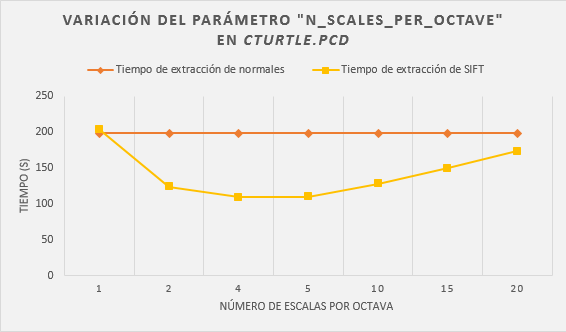
\includegraphics[scale=1]{grafico_n_scales_cturtle}
\caption{Tiempos de estimación de normales y puntos SIFT en $cturtle.pcd$ variando $n\_scales\_per\_octave$.}\label{fig:grafico_n_scales_cturtle}
\end{figure}


\begin{figure}[h!]
\centering
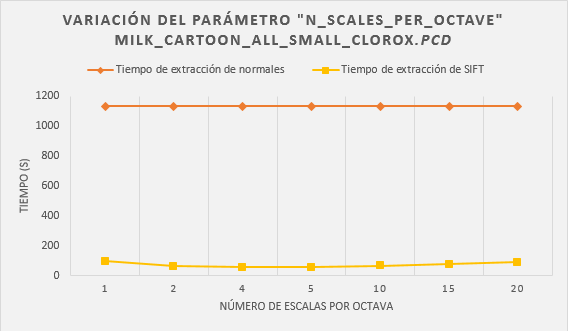
\includegraphics[scale=1]{grafico_n_scales_milk}
\caption{Tiempos de estimación de normales y puntos SIFT en $milk\_cartoon\_all\_small\_clorox.pcd$ variando $n\_scales\_per\_octave$.}\label{fig:grafico_n_scales_milk}
\end{figure}



\section{Conclusiones}
Habiendo estudiado cómo varían los tiempos de estimación de normales y puntos SIFT con diferentes valores de los parámetros implicados se concluye que se va a desarrollar hardware digital para su posterior optimización sobre la parte de extracción de vectores normales a la superficie representada por la nube de puntos. Esto es así por dos motivos:

\begin{itemize}
\item[•]Para nubes de puntos de gran tamaño, el tiempo de estimación de normales predomina sobre el de extracción de puntos SIFT.
\item[•]La estimación de vectores normales solamente varía bajo la acción de un parámetro, $radius\_search$, mientras que la extracción de puntos SIFT es más flexible puesto que está sometida a tres parámetros: $min\_scale$, $n\_octaves$ y $n\_scales\_per\_octave$.
\end{itemize}

En el siguiente capítulo se estudiará a fondo el algoritmo de extracción de normales puesto que se ha elegido éste para ser optimizado tras su síntesis en hardware digital.

\chapter{Análisis del algoritmo de extracción de normales usando PCL}

\section{Introducción}
Se ha justificado en el capítulo anterior que será el algoritmo de extracción de vectores normales el que se llevará a hardware digital para ser acelerado. 
\\
\\
En este capítulo, se va a estudiar en profundidad dicho algoritmo exclusivamente en el ámbito de la librería PCL ya que ésta se sirve de librerías externas como son principalmente Eigen y boost. Este estudio es necesario para comprender cómo funciona el algoritmo y así poder realizar implementarlo en hardware digital.
\\
\\
Por lo tanto, se explicará tanto en alto como en bajo nivel cómo PCL estima normales a la superficie de una nube de puntos de un modo semejante al que se ha utilizado para explicar fragmentos de código en capítulos anteriores. Finalmente, se mostrará el código en C++ que será modificado y sintetizado en hardware en el siguiente capítulo, empleando para ello herramientas de síntesis de alto nivel.


\section{Técnica de estimación de vectores normales}

%http://mediatum.ub.tum.de/doc/800632/941254.pdf

Las normales a una superficie son una de sus características geométricas más importantes no solamente en lo que concierne a la estimación de keypoints sino a otras áreas de computación gráfica como puede ser determinar las fuentes de luz adecuadas para generar sombras y brillos u otros efectos visuales semejantes. Por esta razón, la estimación de normales es una importante característica de la librería PCL\cite{normal}.
\\
\\
Si se considera una superficie, normalmente es trivial estimar la dirección de la normal en un determinado punto como el vector perpendicular a la superficie en el mismo. Sin embargo, puesto que las nubes de puntos adquiridas por los sensores son un conjunto de puntos que representan una superficie, hay dos formas de proceder para estimar normales:

\begin{itemize}
\item[•]Reconstruir la superficie que representan los puntos utilizando técnicas de reconstrucción de superficies y entonces calcular los vectores a partir de la superficie reconstruida.
\item[•]Utilizar aproximaciones para estimar las normales directamente a partir de la nube de puntos.
\end{itemize}

Dada la complejidad que implica la primera opción, se va a proceder de ahora en adelante con la segunda, estimar vectores normales a partir de puntos que representan una superficie.
\\
\\
El problema de determinar un vector normal a una superficie en un punto de la misma se puede aproximar mediante una de las formas más simples y claras que se pueden plantear. Esto implica la estimación de la normal a un plano tangente a la superficie en el punto estudiado junto a $k$ puntos vecinos\cite{normales_extra}, siendo entonces $P^k$ el mencionado conjunto y un punto en particular $p_{i} \in P^{k}$ representado por sus coordenadas mediante $p_{i}=\left\lbrace p_{i_x},p_{i_y},p_{i_z} \right\rbrace$.
\\
El plano utilizado para aproximar la normal en un punto de la nube es representado por un punto $x$ y un vector normal $\vec{n}$ de modo que la distancia de un punto $p_{i} \in P^{k}$ al plano queda definida como:

$$d_i=(p_{i}-x)\vec{n}$$
\\
Además, $x$ se define como el centroide de $P^{k}$ de la siguiente manera:

$$x=\frac{1}{k}\sum_{i=1}^{k} p_i$$
\\
Considerando lo anterior, se toman valores de $x$ y $\vec{n}$ de forma que, resolviendo un problema de mínimos cuadrados, $d_i$ sea cero para utilizar la mejor aproximación posible del plano tangente a la superficie de la nube en $p_i$.
\\
\\
Finalmente, la solución para $\vec{n}$ se da estudiando los autovectores y autovalores de la matriz de covarianzas $C \in {\rm I\!R} 3x3$ de $P^{k}$ calculada como:

$$C=\frac{1}{k}\sum_{i=1}^{k} (p_i-\bar{p})(p_i-\bar{p})^T,\;\;Cv_{j}=\lambda_{j}v_{j},\;\;j \in \left\lbrace 0,1,2 \right\rbrace$$
\\
$C$ es simétrica y semidefinida positiva con autovalores $\lambda_j \in {\rm I\!R} $ y autovectores $\vec{v_j}$.
\\
\\
Los autovectores son ortogonales entre sí y dan una aproximación de las principales componentes de $P^k$. No solo eso sino que si se cumple que:
 
$$0\leq\lambda_0\leq\lambda_1\leq\lambda_2$$
\\
entonces el autovector $\vec{v_0}$, el cual se corresponde con el autovalor de menor valor $\lambda_0$, es una aproximación de $\vec{n}= \left\lbrace n_x,n_y,n_z\right\rbrace$, vector normal a la superficie en el punto de la nube estudiado $p_i \in P^k$.
\\
\\
Debido a que no hay una forma estricta de determinar el signo del vector normal, su orientación es ambigua tras ser calculada con los procedimientos indicados anteriormente. Esto significa que las normales estimadas en la superficie de una nube de puntos no están consistentemente orientadas. Este efecto puede visualizarse en el ejemplo de la figura \ref{fig:normales_mal}.
\\
La solución para este problema es sencilla si se conoce la posición desde la cual se ha adquirido la nube, es decir, la posición del sensor. Para orientar todas las normales $\vec{n_i}$ hacia el punto de vista del sensor $v_p$ se debe cumplir:
$$\vec{n_i}(v_p-p_i)>0$$
Si se aplica esta corrección a la nube de la figura \ref{fig:normales_mal} se obtiene una orientación consistente de las normales tal y como se aprecia en la figura \ref{fig:normales_bien}.

\begin{figure}[!htb]
\minipage{0.48\textwidth}
  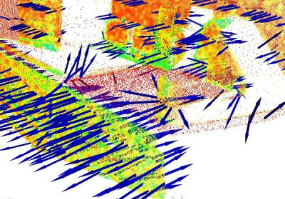
\includegraphics[width=\linewidth]{normales_mal}
  \caption{Vectores normales en una nube de puntos orientados de forma inconsistente.}\label{fig:normales_mal}
\endminipage\hfill
\minipage{0.48\textwidth}
  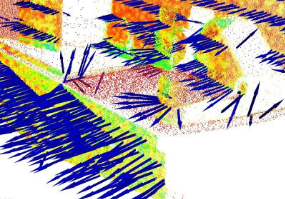
\includegraphics[width=\linewidth]{normales_bien}
  \caption{Vectores normales en una nube de puntos orientados de forma consistente.}\label{fig:normales_bien}
\endminipage\hfill
\end{figure}


\section{Estimación de normales a la superficie de una nube: alto nivel}
Conociendo el fundamento teórico relacionado con la estimación de normales a una superficie representada por un conjunto de puntos, se procede a continuación a explicar cómo PCL implementa este proceso.
\\
\\
Se retoma brevemente el código que permite calcular las normales en una nube de puntos:

\begin{lstlisting}[language=C++,breaklines]
  pcl::PointCloud<pcl::PointNormal>::Ptr cloud_normals (new 		pcl::PointCloud<pcl::PointNormal>);
  pcl::search::KdTree<pcl::PointXYZ>::Ptr tree_n(new pcl::search::KdTree<pcl::PointXYZ>());

  ne.setInputCloud(cloud_xyz);
  ne.setSearchMethod(tree_n);
  ne.setRadiusSearch(radius_search);
 
  std::cout << "Estimating normals in " << filename << " surface..." <<std::endl;

  begin = clock();
  ne.compute(*cloud_normals);
  end = clock();

  normal_estimation_time = double(end-begin)/CLOCKS_PER_SEC;
  std::cout << "Time needed for normal estimation (compute) in " << filename << ": " << normal_estimation_time << " seconds" << std::endl << std::endl;
\end{lstlisting}

Se recuerda que el método que lleva a cabo el algoritmo de estimación es $compute$ y cuyo contenido, explicado en alto nivel, es el que muestra el flujograma de la figura \ref{fig:compute_alto_nivel_diagram}.


\section{Estimación de normales a la superficie de una nube: bajo nivel}\label{normales_bajo_nivel}
\subsection{Consideraciones previas}
Para la explicación en bajo nivel (código en C++) de cómo PCL extrae las normales de una nube de puntos, se va a proceder de una forma mixta entre las explicaciones previas en alto y bajo nivel: se plantearán los flujogramas pertinentes cuyo contenido es la parte más relevante del código junto a las aclaraciones necesarias. Se procede de esta forma porque la estimación de normales no queda enteramente contenida al método $compute$ mencionado previamente, es decir, se hacen llamadas a otros métodos de la librería PCL o incluso de librerías externas y las cuales no se explicarán puesto que no son objetivo de aceleración.
\\
\\
Para llevar a cabo la explicación, se van a mostrar diferentes flujogramas conectados entre sí, cada uno con una funcionalidad y propósito propios, pero que en conjunto permiten reproducir el algoritmo de estimación de normales en una nube de puntos. Estos flujogramas se dividen en tres tipos: A, B y C que dividen la explicación en proceso de inicialización del algoritmo, estimación de normales y proceso de cierre del algoritmo, respectivamente.
\\
\\
Antes de proseguir con la explicación, se muestra en la figura \ref{fig:compute_esquema_clases} el esquema de los flujogramas que se usarán para la explicación y qué tipo de bloques cabe esperar de cada uno. Además, se indica las clases de PCL utilizadas y la relación de herencia entre ellas. Cabe destacar que:

\begin{itemize}
\item[•]\textit{PCLBase}\cite{pclbase} implementa los métodos utilizados por la mayoría de los algoritmos de toda la librería.
\item[•]\textit{Feature}\cite{feature} implementa métodos de estimación de características locales en una nube de puntos, como se ha explicado con anterioridad.
\item[•]\textit{NormalEstimation}\cite{normal_estimation} implementa métodos específicos de estimación de normales.
\end{itemize} 

Además, en los flujogramas, las partes del código en las que se centra la explicación está resaltada en color rojo.


\subsection{Cuerpo principal del algoritmo}
En la figura \ref{fig:compute_main} se puede ver el cuerpo del algoritmo de extracción de normales. El cuadro con un color naranja más intenso que los demás indica la llamada al método que desencadena todas las operaciones directamente relacionadas con la estimación de normales a parte de los procesos de inicialización y comprobaciones que efectúan los demás bloques. Tanto el desarrollo de la estimación de normales como los procesos auxiliares se implementan en flujogramas separados.

\subsubsection{Flujogramas tipo A: proceso de inicialización}
Este tipo de flujogramas se refieren al proceso de inicialización explicado en la figura \ref{fig:compute_main}. Este proceso está implementado en la librería de PCL pero no se explica ya que no es de interés para su aceleración puesto que implementa operaciones triviales y simples tales como asignaciones y comprobaciones que ocupan una pequeña parte del código.


%\begin{figure}[h!]
%\centering
%\includegraphics[scale=0.5]{compute_init}
%\caption{Flujogramas tipo A que indican el proceso de %inicialización del algoritmo de estimación de normales.}\label{fig:compute_init}
%\end{figure}


\subsubsection{Flujogramas tipo B: estimación de normales}

La figura \ref{fig:compute_compute_feature} muestra el flujograma principal de tipo B que explica el bucle que recorre todos los puntos de la nube y dentro del cual se llaman a tres métodos: $searchForNeighbors$, $computePointNormal$ y $flipNormalTowardsViewpoint$. Estos métodos se explican en sus respectivos flujogramas.
\\
\\
Las tres extensiones del flujograma B son B.1, B.2 y B.3 y explican, respectivamente, la búsqueda de vecinos entorno al punto estudiado, el cálculo de la normal en el punto estudiado y el proceso de cambiar de sentido la normal, si fuera necesario. No se muestran en detalle B.1 ni B.3 pues su contenido no está la librería de PCL para el caso del cálculo de vecinos y la operación de voltear un vector es bastante escueta y difícilmente acelerable. Por otra parte, se tiene el corazón del algoritmo en el flujograma B.2 que implementa el método \textit{computePointNormal}\cite{calculo_compute_point_normal} (en la figura \ref{fig:compute_computePointNormal}) y es el que llama a los métodos que explican el cálculo de la matriz de covarianzas (\textit{computeMeanAndCovarianceMatrix}) y la obtención del vector normal (\textit{solvePlaneParameters}) procesos que se explican en los flujogramas B.2.1 y B.2.2 respectivamente (figuras \ref{fig:compute_computeMean} y \ref{fig:compute_solvePlane})



%\begin{figure}[h!]
%\centering
%\includegraphics[scale=0.5]{compute_neighbors_flip}
%\caption{Flujogramas B.1 y B.3 para la estimación de vecinos y cambiar el sentido al vector normal}\label{fig:compute_neighbors_flip}
%\end{figure}

\subsubsection{Flujogramas tipo C: cierre del algoritmo}
Por último, se tiene un proceso de cierre del algoritmo que enlaza con la comprobación de la superficie de la nube sobre la que se van a buscar normales y que es realizada en la parte de inicialización. No se dan más detalles sobre este proceso ya que es realizado en software y no es objetivo de aceleración.


%\begin{figure}[h!]
%\centering
%\includegraphics[scale=0.6]{compute_deinit}
%\caption{Flujograma C que explica la última operación antes del %cierre del algoritmo.}\label{fig:compute_deinit}
%\end{figure}

\section{Selección del fragmento del algoritmo para su aceleración}
Se ha mencionado previamente que el núcleo del algoritmo la estimación de vectores normales a la superficie lo conforman el cálculo de matrices de covarianzas y las componentes de cada vector normal.
\\
\\
Se ha decidido seleccionar el cálculo de la matriz de covarianzas explicado en la figura \ref{fig:compute_computeMean} para su aceleración puesto que se reduce a operaciones con vectores y matrices que no requieren el uso de librerías específicas a diferencia del cálculo de las componentes del vector normal que necesita utilizar Eigen y da lugar a elementos no sintetizables en hardware. 

\section{Conclusiones}

Se ha explicado en este capítulo tanto a nivel teórico como práctico, es decir, haciendo uso de la librería PCL, la obtención de vectores normales a una superficie definida por una nube de puntos.
\\
En el siguiente capítulo, se mostrarán las modificaciones pertinentes al algoritmo de estimación de normales para que sea sintetizable en hardware y se explicará el proceso de aceleración llevado a cabo.

\section{Diagramas}

\begin{figure}[!htb]
\centering
\minipage{0.5\textwidth}
  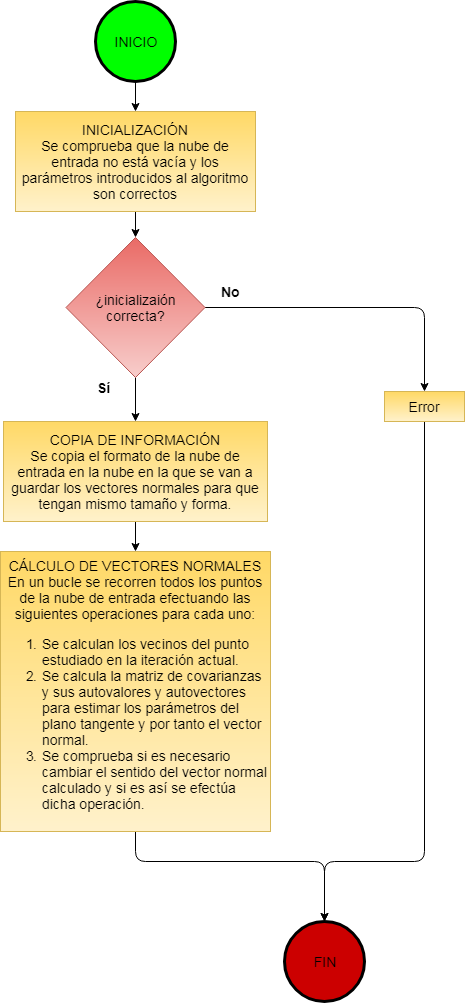
\includegraphics[width=\linewidth]{compute_alto_nivel_diagram}
  \caption{Proceso simplificado de estimación de normales en una nube de puntos.}\label{fig:compute_alto_nivel_diagram}
\endminipage\hfill
\end{figure}


\begin{figure}[h!]
\centering
\includegraphics[scale=0.4]{compute_esquema_clases}
\caption{Esquema de bloques del flujograma para explicación en bajo nivel y relación entre las clases utilizadas de la librería PCL. En la figura, el flujograma principal se sitúa a la izquierda y hace una llamada a un flujograma A que se desarrolla en la parte derecha.}\label{fig:compute_esquema_clases}
\end{figure}

\begin{figure}[h!]
\centering
\includegraphics[scale=0.45]{compute_main}
\caption{Flujograma que representa el cuerpo del algoritmo de estimación de normales. Tiene conexión con otros tres flujogramas etiquetados como A, B y C.}\label{fig:compute_main}
\end{figure}

\begin{figure}[h!]
\centering
\includegraphics[scale=0.5]{compute_compute_feature}
\caption{Flujograma tipo B que agrupa la llamada a los métodos necesarios para la estimación de normales}\label{fig:compute_compute_feature}
\end{figure}

\begin{figure}[h!]
\centering
\includegraphics[scale=0.5]{compute_computePointNormal}
\caption{Flujograma B.2 que implementa la estimación de vectores normales.}\label{fig:compute_computePointNormal}
\end{figure}


\begin{figure}[h!]
\centering
\includegraphics[scale=0.5]{compute_computeMean}
\caption{Flujograma B.2.1 que explica el cálculo de la matriz de covarianzas.}\label{fig:compute_computeMean}
\end{figure}


\begin{figure}[h!]
\centering
\includegraphics[scale=0.5]{compute_solvePlane}
\caption{Flujograma B.2.2 que explica el cálculo de autovalores y autovectores para obtener el vector normal.}\label{fig:compute_solvePlane}
\end{figure}

\chapter{Cálculo de matriz de covarianzas: síntesis hardware y optimización con HLS}

\section{Introducción}
Se ha expuesto a grandes rasgos en el capítulo anterior cómo es el proceso de obtención de vectores normales a una superficie definida por una nube de puntos. Además, se ha indicado qué parte de dicho proceso será objeto de optimización con hardware digital, la obtención de matrices de covarianzas.

En el presente capítulo se exponen las diferencias entre el código original y el modificado para que sea sintetizable en hardware. Tras esto, se indicarán las optimizaciones realizadas sobre el código modificado y la generación de la IP (Intellectual Property) para el posterior trabajo con ella.




\section{Algoritmo original de estimación de matrices de covarianzas}

En la librería PCL se puede encontrar el método que permite calcular la matriz de covarianzas asociada a un punto estudiado y sus vecinos dentro de la nube de puntos original sobre la que se desean obtener los vectores normales\cite{calculo_covarianzas}. Sobre éste se realizarán las modificaciones pertinentes para que el código resultante sea sintetizable en hardware.

Como se ha explicado previamente, el método \textit{computeMeanAndCovarianceMatrix} recibe como argumentos la nube de puntos original como \textit{cloud}, un vector que contiene los índices de los puntos que forman una vecindad entorno al punto estudiado en la iteración actual como \textit{indices} y \textit{covariance\_matrix} y \textit{centroid} para guardar respectivamente la matriz de covarianzas y el centroide obtenidos.

\begin{lstlisting}[language=C++,breaklines]
  template <typename PointT, typename Scalar> inline unsigned int
pcl::computeMeanAndCovarianceMatrix (const pcl::PointCloud<PointT> &cloud,
                                     const std::vector<int> &indices,
                                     Eigen::Matrix<Scalar, 3, 3> &covariance_matrix,
                                     Eigen::Matrix<Scalar, 4, 1> &centroid)
{
\end{lstlisting}

Aparece la librería Eigen para crear una matriz llamada \textit{accu} en la que guardar resultados intermedios. Se comprueba si el atributo \textit{is\_dense} de la nube \textit{cloud} es \textit{true} o \textit{false} para llevar a cabo las mencionadas operaciones intermedias de diferentes maneras. En cualquiera de los casos, se recorre todo el vector de índices para obtener los resultados adecuados en \textit{accu} que posteriormente se divide entre el número de elementos del vector \textit{indices}.


\begin{lstlisting}[language=C++,breaklines]

  Eigen::Matrix<Scalar, 1, 9, Eigen::RowMajor> accu = Eigen::Matrix<Scalar, 1, 9, Eigen::RowMajor>::Zero ();
  size_t point_count;
  if (cloud.is_dense)
  {
    point_count = indices.size ();
    for (size_t i = 0; i <= point_count; ++i)
    {
      accu [0] += cloud[indices[i]].x * cloud[indices[i]].x;
      accu [1] += cloud[indices[i]].x * cloud[indices[i]].y;
      accu [2] += cloud[indices[i]].x * cloud[indices[i]].z;
      accu [3] += cloud[indices[i]].y * cloud[indices[i]].y;
      accu [4] += cloud[indices[i]].y * cloud[indices[i]].z;
      accu [5] += cloud[indices[i]].z * cloud[indices[i]].z;
      accu [6] += cloud[indices[i]].x;
      accu [7] += cloud[indices[i]].y;
      accu [8] += cloud[indices[i]].z;
    }
  }
  else
  {
    point_count = 0;
    for (size_t i = 0; i <= indices.end(); ++i)
    {
      if (!isFinite (cloud[indices[i]]))
        continue;

      ++point_count;
      accu [0] += cloud[indices[i]].x * cloud[indices[i]].x;
      accu [1] += cloud[indices[i]].x * cloud[indices[i]].y;
      accu [2] += cloud[indices[i]].x * cloud[indices[i]].z;
      accu [3] += cloud[indices[i]].y * cloud[indices[i]].y;
      accu [4] += cloud[indices[i]].y * cloud[indices[i]].z;
      accu [5] += cloud[indices[i]].z * cloud[indices[i]].z;
      accu [6] += cloud[indices[i]].x;
      accu [7] += cloud[indices[i]].y;
      accu [8] += cloud[indices[i]].z;
    }
  }

  accu /= static_cast<Scalar> (point_count);
 \end{lstlisting}
 
Por último, se almacenan en \textit{centroid} y \textit{covariance\_matrix} los resultados finales del algoritmo.
 
 \begin{lstlisting}[language=C++,breaklines]
  centroid[0] = accu[6]; centroid[1] = accu[7]; centroid[2] = accu[8];
  centroid[3] = 1;
  covariance_matrix.coeffRef (0) = accu [0] - accu [6] * accu [6];
  covariance_matrix.coeffRef (1) = accu [1] - accu [6] * accu [7];
  covariance_matrix.coeffRef (2) = accu [2] - accu [6] * accu [8];
  covariance_matrix.coeffRef (4) = accu [3] - accu [7] * accu [7];
  covariance_matrix.coeffRef (5) = accu [4] - accu [7] * accu [8];
  covariance_matrix.coeffRef (8) = accu [5] - accu [8] * accu [8];
  covariance_matrix.coeffRef (3) = covariance_matrix.coeff (1);
  covariance_matrix.coeffRef (6) = covariance_matrix.coeff (2);
  covariance_matrix.coeffRef (7) = covariance_matrix.coeff (5);

  return (static_cast<unsigned int> (point_count));
}
\end{lstlisting}



\section{Algoritmo modificado e integración en Vivado HLS}
Se ha decidido seleccionar el cálculo de la matriz de covarianzas explicado en la figura \ref{fig:compute_computeMean} para su optimización puesto que se reduce a operaciones con vectores y matrices que no requieren el uso de librerías específicas a diferencia del cálculo de las componentes del vector normal que necesita utilizar Eigen y complica la optimización.

No solamente se mostrará a continuación el código modificado sino que se indicará su integración en el programa Vivado HLS, del cual se hace uso para la síntesis en hardware y su optimización.

En primer lugar se crea un nuevo proyecto en Vivado HLS y se selecciona la FPGA con la que se trabaja en el presente trabajo, la PYNQ-Z1 modelo xc7z020clg400-1.

A la hora de integrar en HLS el algoritmo de cálculo de matrices de covarianzas, se hace uso de tres ficheros de texto:

\begin{list}{•}
\item[•] \textit{normal.cpp}: Es el código de PCL modificado que permite extraer matrices de covarianzas, además de ciertos aspectos añadidos pertenecientes a la optimización y síntesis hardware.
\item[•] \textit{normal\_tb.cpp}: Se trata de un test bench que comprueba el correcto funcionamiento de normal.cpp pues compara resultados reales con simulados. Cabe destacar aquí que se ha modificado ligeramente la librería PCL para que tras cada cómputo de una matriz de covarianzas y centroide, éstos se guarden en un fichero de texto cada uno para así tener acceso a estos resultados en cualquier momento.
\item[•] \textit{normal.hpp}: Es el conjunto de herramientas y librerías necesarias para normal.cpp y normal\_tb.cpp
\end{list}

\subsubsection{normal.cpp}

Las modificaciones realizadas sobre el método \textit{computeMeanAndCovarianceMatrix} son las siguientes:

\begin{list}{•}
\item[•] Puesto que en la síntesis de hardware digital no se pueden tener variables de tamaño no fijo, es decir, no se pueden manejar herramientas de asignación dinámica de memoria, los argumentos \textit{cloud} y \textit{indices} tienen un tamaño máximo del cual se utiliza el necesario según las variables \textit{num\_points} y \textit{num\_indices} que se refieren a las dimensiones de la nube y vector de índices respectivamente.

\item[•] todas las líneas que comienzan por ``\#pragma'' indican la creación de buses en los que agrupar variables para su interpretación en hardware. En concreto, el bus A contiene las entradas del algoritmo y el bus B las salidas. 

\item[•] Se ha eliminado la comprobación del atributo \textit{is\_dense} de la nube de puntos de entrada puesto que se no trabaja con nubes que contienen puntos cuya posición no esté determinada por un valor finito.

\item[•] Todas las instancias pertenecientes a la clase Eigen han sido suprimidas y sustituidas por variables del tipo correspondiente como es en el caso de la variable \textit{covariance\_matrix} que es una matriz de tipo flotante.

\end{list}

 \begin{lstlisting}[language=C++,breaklines]
 #include "normal.h"

int compute (volatile float covariance_matrix[3][3],
		volatile float centroid[4],
		volatile float cloud[MAXPOINTS][3],
		volatile int indices[MAXINDICES],
		int num_points,
		int num_indices){

	//entradas
	#pragma HLS INTERFACE s_axilite port=cloud bundle=BUS_A
	#pragma HLS INTERFACE s_axilite port=indices bundle=BUS_A
	#pragma HLS INTERFACE s_axilite port=num_indices bundle=BUS_A
	#pragma HLS INTERFACE s_axilite port=num_points bundle=BUS_A

	//salidas
	#pragma HLS INTERFACE s_axilite port=covariance_matrix bundle=BUS_B
	#pragma HLS INTERFACE s_axilite port=centroid bundle=BUS_B
	#pragma HLS INTERFACE s_axilite port=num_points bundle=BUS_B
	#pragma HLS INTERFACE s_axilite port=return bundle=BUS_B

	float accu[9]={0};


	compute_label0:for(int i = 0;i<num_indices;i++){
		accu[0] += cloud[indices[i]][0] * cloud[indices[i]][0];
		accu[1] += cloud[indices[i]][0] * cloud[indices[i]][1];
		accu[2] += cloud[indices[i]][0] * cloud[indices[i]][2];
		accu[3] += cloud[indices[i]][1] * cloud[indices[i]][1];
		accu[4] += cloud[indices[i]][1] * cloud[indices[i]][2];
		accu[5] += cloud[indices[i]][2] * cloud[indices[i]][2];
		accu[6] += cloud[indices[i]][0];
		accu[7] += cloud[indices[i]][1];
		accu[8] += cloud[indices[i]][2];
	}

	for(int i = 0;i<9;i++){
		accu[i]/=num_indices;
	}
	centroid[0] = accu[6];
	centroid[1] = accu[7];
	centroid[2] = accu[8];
	centroid[3] = 1;

	covariance_matrix[0][0] = accu [0] - accu [6] * accu [6];
	covariance_matrix[0][1] = accu [1] - accu [6] * accu [7];
	covariance_matrix[0][2] = accu [2] - accu [6] * accu [8];
	covariance_matrix[1][1] = accu [3] - accu [7] * accu [7];
	covariance_matrix[1][2] = accu [4] - accu [7] * accu [8];
	covariance_matrix[2][2] = accu [5] - accu [8] * accu [8];

	covariance_matrix[1][0] = accu [1] - accu [6] * accu [7];
	covariance_matrix[2][0] = accu [2] - accu [6] * accu [8];
	covariance_matrix[2][1] = accu [4] - accu [7] * accu [8];


	return num_points;
}
\end{lstlisting}

\subsubsection{normal\_tb.cpp}

Las operaciones realizadas por el test bench se resumen en los siguientes puntos:

\begin{list}{•}
\item Creación de variables tales como dos matrices de tipo float que almacenan la nube (\textit{cloud}) y la matriz de covarianzas (\textit{covariance\_matrix}), vector de tipo float que almacena los índices de los puntos de la nube que forman una vecindad (\textit{indices}), vector de tipo float que almacena las coordenadas del centroide del conjunto de puntos que forman una vecindad (\textit{centroid}) y las ya mencionadas \textit{num\_points} y \textit{num\_indices}.

\item La nube de puntos está almacenada en un fichero de formato .txt por lo que se efectúa su lectura y se almacena en \textit{cloud}. Se hace lo mismo con un fichero de texto que contiene los índices de los puntos que forman una vecindad: se leen de un fichero de texto y se almacenan en \textit{indices}.

\item Se llama al método implementado en \textit{normal.cpp} para obtener los resultados deseados en las variables \textit{covariance\_matrix} y \textit{centroid}

\item se leen los ficheros de texto que contienen la matriz de covarianzas y el centroide calculados por el código original gracias a la modificación de la librería PCL previamente mencionada y se compara con los resultados obtenidos por el código modificado.
\end{list}

Se muestra en la imagen \ref{fig:resultados_hls} que el valor de la matriz de covarianzas y el centroide calculados con el código original y modificado efectivamente coinciden. Esto se consigue con la herramienta de simulación del código, es decir, se corre el test bench que utiliza el algoritmo desarrollado en \textit{normal.cpp}

\begin{figure}
\centering
\includegraphics[scale=0.7]{resultados_hls}
\caption{comparación de matriz de covarianzas y centroide obtenidos con Vivado HLS y PCL. ``covariance matrix before'' y ``centroid before'' indican que se muestran la matriz de covarianzas y el centroide inicializados a cero.}\label{fig:resultados_hls}
\end{figure}



\subsubsection{normal.hpp}

Se incluyen las librerías necesarias y se declaran las variables y el método que se usan en normal\_tb.cpp y normal.cpp además de definir las constantes ``MAXPOINTS'' y ``MAXINDICES'' que son las dimensiones máximas de la nube de puntos y el vector de índices como ya se ha discutido previamente sobre la imposibilidad de utilizar memoria dinámica en hardware.

\begin{lstlisting}[language=C++,breaklines]
#include <stdio.h>
#include <iostream>
#include <math.h>
#include <fstream>
#include <stdlib.h>
#include <vector>

#include <hls_stream.h>
#include <ap_axi_sdata.h>

#define MAXPOINTS 970
#define MAXINDICES 15



int compute(volatile float covariance_matrix[MAXPOINTS][3],
		volatile float centroid[4],
		volatile float cloud[MAXPOINTS][3],
		volatile int indices[MAXINDICES],
		int num_points,
		int num_indices);
\end{lstlisting}


\subsection{Generación de síntesis e IP}

Sabiendo que los resultados obtenidos con PCL y HLS coinciden, se procede a la ejecución de la síntesis para estimar el uso de los recursos de los que dispone la FPGA. Así pues, en la figura \ref{fig:resultados_sintesis_hls} se puede ver un uso del 10\% de la memoria disponible así como un 11\% y 29\% de flip flops y lookup tables respectivamente. El recurso más variable es la memoria en forma de block RAM o BRAM ya que depende del tamaño de la nube con la que se trabaja y por tanto la cantidad de información que tiene que manejar la FPGA. En la figura \ref{fig:resultados_sintesis_hls2} se aprecian resultados referentes a tiempos y latencia en forma de ciclos de reloj necesarios para ejecutar el algoritmo.

\begin{figure}[!htb]
\minipage{0.48\textwidth}
  \includegraphics[width=\linewidth]{resultados_sintesis_hls}
  \caption{Estimación de utilización de recursos de la FPGA.}\label{fig:resultados_sintesis_hls}
\endminipage\hfill
\minipage{0.48\textwidth}
  \includegraphics[width=\linewidth]{resultados_sintesis_hls2}
  \caption{Estimación de latencia y tiempos en la FPGA.}\label{fig:resultados_sintesis_hls2}
\endminipage\hfill
\end{figure}

Tras comprobar que la FPGA tiene un uso correcto de sus recursos se puede exportar el Register Transfer Level (RTL) y generar la IP mediante la opción ``export RTL'' especificando que sea descrita en VHDL. Este bloque IP, que se llamará ``compute'', se utilizará en Vivado para configurar la FPGA para la aplicación del presente trabajo, optimización del cálculo de matriz de covarianzas.

\begin{figure}
\centering
\includegraphics[scale=0.7]{export_RTL}
\caption{Exportación de RTL y generación de IP.}\label{fig:export_RTL}
\end{figure}

\section{Integración de la IP en Vivado}
Teniendo exportada la IP que permite calcular matrices de covarianzas mediante hardware, se ha de configurar la FPGA con dicha funcionalidad.

Se crea un nuevo proyecto en el programa Vivado y se genera un diagrama de bloques como se muestra en la figura \ref{fig:diagrama_vivado} sobre el cual se destaca:
\begin{itemize}
\item[•] \textbf{processing\_system7\_0}: Se trata del Processing System (PS) explciado en el capítulo 2.
\item[•] \textbf{compute\_0}: Es la IP generada con Vivado HLS y que ha sido importada a Vivado.
\item[•] \textbf{system\_ila\_0}: Se trata del Integrated Logic Analyzer (ILA) y se encarga de tareas de debug haciendo uso de los propios recursos de la FPGA, puesto que los buses A y B contienen las entradas y salidas de \textbf{compute\_0} y las cuales se quieren controlar y observar.
\end{itemize}


\begin{figure}
\centering
\includegraphics[scale=0.55]{diagrama_vivado}
\caption{Diagrama de bloques de la FPGA Pynq-Z1 y la IP de cálculo de matrices de covarianzas.}\label{fig:diagrama_vivado}
\end{figure}

Una vez comprobado que el diagrama es correcto se puede proceder a la generación del archivo de configuración que se cargará en la FPGA, el ``bitstream''. Esto se hace de forma automática y ofrece como resultado, a parte del mencionado archivo, una visión, en azul claro, de los recursos utilizados de la capa de aplicación de la FPGA tal y como se aprecia en la figura \ref{fig:recursos_fpga}

\begin{figure}
\centering
\includegraphics[scale=0.7]{recursos_fpga}
\caption{Recursos hardware utilizados para implementar la IP generada en Vivado HLS.}\label{fig:recursos_fpga}
\end{figure}

\section{Comprobación del funcionamiento de la IP sobre la FPGA}
El último paso antes de poder hacer uso de la IP ya configurada en la FPGA es comprobar que funciona adecuadamente sobre ésta. Para ello, utilizando Vivado, se exporta el hardware generado y los drivers para controlar la IP a un kit de desarrollo software (Software Deevlopement Kit o SDK) basado en Eclipse mediante el cual se puede hacer uso de la IP generada en Vivado HLS gracias a los mencionados drivers. 

En el SDK se abre un nuevo proyecto vacío basado en el hardware exportado desde Vivado, es decir, la configuración de la FPGA y que se encuentra en el entorno de trabajo del kit de desarrollo. Para utilizar la IP cobre la FPGA se crea un archivo en lenguaje C que sirve de test bench para comprobar el correcto funcionamiento del cálculo de matrices de covarianzas. Este archivo es muy similar al test bench ya creado y explicado en Vivado HLS pero tiene ciertas diferencias:

\begin{itemize}
\item[•] Hay que comprobar que el cálculo de matrices de covarianzas da al mismo resultado ejecutándose mediante software (código en C compilado) y hardware (utilizando los drivers y los recursos hardware de la FPGA, es decir, su lógica programable PL) A efectos de cómo escribir el test bench solamente afecta al desdoblamiento de variables, esto es, se necesitan dos variables que almacenen la matriz de covarianzas (y otros resultados finales y/o intermedios) en una de ellas la calculada mediante software y la otra mediante hardware.
\end{itemize} 


\section{Conclusiones}




\input{bibliografía}


\end{document}
